\chapter{Experimental Results}
    \label{chap:exp_sim_res}
    \begin{itemize}
        \item \textbf{$N = 5$ Circular Formation:}
            \begin{table}[H]
                \caption{Simulation Results for N=5 Circular Formation.}
                \label{n_5_circ}
                \centering
                \renewcommand{\arraystretch}{1.2}
                \begin{tabular}{|l|c|c|c|c|c|}
                \hline
                                            & \( SR \ [\%] \) & \( \overline{L} \ [\mathrm{m}] \) & \( \overline{t} \ [\mathrm{s}] \) & \( \overline{t}_{\text{max}} \ [\mathrm{s}] \) & \( \overline{v} \ [\mathrm{m/s}] \)     \\ \hline
                RBL 2D                      & 100.00          & 21.06 $\pm$ 0.10                  & $\mathbf{25.15} \boldsymbol{\pm} \mathbf{0.21}$                  & $\mathbf{25.15} \boldsymbol{\pm} \mathbf{0.19}$                               & $\mathbf{0.83} \boldsymbol{\pm} \mathbf{0.01}$                         \\ \hline
                RBL 3D                      & 100.00          & 20.77 $\pm$ 0.29                  & 26.04 $\pm$ 0.51                  & 26.79 $\pm$ 0.27                               & 0.79 $\pm$ 0.02                         \\ \hline
                RBL 3D\(_{\text{clipped}}\) & 100.00          & $\mathbf{20.60} \boldsymbol{\pm} \mathbf{0.24}$                  & 26.73 $\pm$ 0.47                  & 27.39 $\pm$ 0.28                               & 0.77 $\pm$ 0.02                         \\ \hline
                RBL 3D\(_{\text{rule}}\)                & 100.00          & 20.97 $\pm$ 0.52                  & 25.54 $\pm$ 0.97                  & 26.72 $\pm$ 0.60                               & 0.81 $\pm$ 0.03                         \\ \hline
                \end{tabular}
            \end{table}
        \item \textbf{$N = 10$ Circular Formation:}
            \begin{table}[H]
                \caption{Simulation Results for N=10 Circular Formation.}
                \label{n_10_circ}
                \centering
                \renewcommand{\arraystretch}{1.2}
                \begin{tabular}{|l|c|c|c|c|c|}
                \hline
                                            & \( SR \ [\%] \) & \( \overline{L} \ [\mathrm{m}] \) & \( \overline{t} \ [\mathrm{s}] \) & \( \overline{t}_{\text{max}} \ [\mathrm{s}] \) & \( \overline{v} \ [\mathrm{m/s}] \)     \\ \hline
                RBL 2D                      & 100.00          & 22.95 $\pm$ 1.64                  & 30.79 $\pm$ 2.28                  & 34.73 $\pm$ 0.77                               & 0.74 $\pm$ 0.07                         \\ \hline
                RBL 3D                      & 100.00          & $\mathbf{22.22} \boldsymbol{\pm} \mathbf{0.89}$                  & 30.05 $\pm$ 2.61                  & 34.39 $\pm$ 4.19                               & 0.73 $\pm$ 0.05                         \\ \hline
                RBL 3D\(_{\text{clipped}}\) & 100.00          & 22.31 $\pm$ 0.69                  & 30.22 $\pm$ 1.83                  & 33.22 $\pm$ 0.93                               & 0.73 $\pm$ 0.04                         \\ \hline
                RBL 3D\(_{\text{rule}}\)                & 100.00          & 22.38 $\pm$ 0.88                  & $\mathbf{28.80} \boldsymbol{\pm} \mathbf{2.30}$                  & $\mathbf{32.35} \boldsymbol{\pm} \mathbf{1.25}$                               & $\mathbf{0.77} \boldsymbol{\pm} \mathbf{0.05}$                         \\ \hline
                \end{tabular}
            \end{table}
        \item \textbf{$N = 15$ Circular Formation:}
            \begin{table}[H]
                \caption{Simulation Results for N=15 Circular Formation.}
                \label{n_15_circ}
                \centering
                \renewcommand{\arraystretch}{1.2}
                \begin{tabular}{|l|c|c|c|c|c|}
                \hline
                                            & \( SR \ [\%] \) & \( \overline{L} \ [\mathrm{m}] \) & \( \overline{t} \ [\mathrm{s}] \) & \( \overline{t}_{\text{max}} \ [\mathrm{s}] \) & \( \overline{v} \ [\mathrm{m/s}] \)     \\ \hline
                RBL 2D                      & 100.00          & 23.56 $\pm$ 1.75                  & 33.89 $\pm$ 2.48                  & 38.75 $\pm$ 1.45                               & 0.69 $\pm$ 0.06                         \\ \hline
                RBL 3D                      & 100.00          & 22.36 $\pm$ 0.97                  & 30.65 $\pm$ 3.07                  & 35.77 $\pm$ 3.72                               & 0.72 $\pm$ 0.07                         \\ \hline
                RBL 3D\(_{\text{clipped}}\) & 100.00          & $\mathbf{22.32} \boldsymbol{\pm} \mathbf{0.81}$                  & 30.69 $\pm$ 2.61                  & 34.50 $\pm$ 0.47                               & 0.72 $\pm$ 0.06                         \\ \hline
                RBL 3D\(_{\text{rule}}\)                & 100.00          & 22.64 $\pm$ 0.95                  & $\mathbf{29.67} \boldsymbol{\pm} \mathbf{2.54}$                  & $\mathbf{34.27} \boldsymbol{\pm} \mathbf{0.88}$                               & $\mathbf{0.76} \boldsymbol{\pm} \mathbf{0.06}$                         \\ \hline
                \end{tabular}
            \end{table}
        \item \textbf{$N = 10$ Spherical Formation:}
            \begin{table}[H]
                \caption{Simulation Results for N=10 Spherical Formation.}
                \label{n_10_sph}
                \centering
                \renewcommand{\arraystretch}{1.2}
                \begin{tabular}{|l|c|c|c|c|c|}
                \hline
                                            & \( SR \ [\%] \) & \( \overline{L} \ [\mathrm{m}] \) & \( \overline{t} \ [\mathrm{s}] \) & \( \overline{t}_{\text{max}} \ [\mathrm{s}] \) & \( \overline{v} \ [\mathrm{m/s}] \)     \\ \hline
                RBL 3D                      & 100.00          & 14.32 $\pm$ 1.52                  & 27.76 $\pm$ 3.06                  & 32.48 $\pm$ 2.26                               & 0.51 $\pm$ 0.05                         \\ \hline
                RBL 3D\(_{\text{rule}}\)                & 100.00          & $\mathbf{14.06} \boldsymbol{\pm} \mathbf{0.97}$                  & $\mathbf{27.17} \boldsymbol{\pm} \mathbf{2.66}$                  & $\mathbf{31.86} \boldsymbol{\pm} \mathbf{1.24}$                               & $\mathbf{0.55} \boldsymbol{\pm} \mathbf{0.06}$                         \\ \hline
                \end{tabular}
            \end{table}
    \end{itemize}

    \begin{figure}[H]
        \centering
        \subfloat[Top-Down View (X-Y)] {
        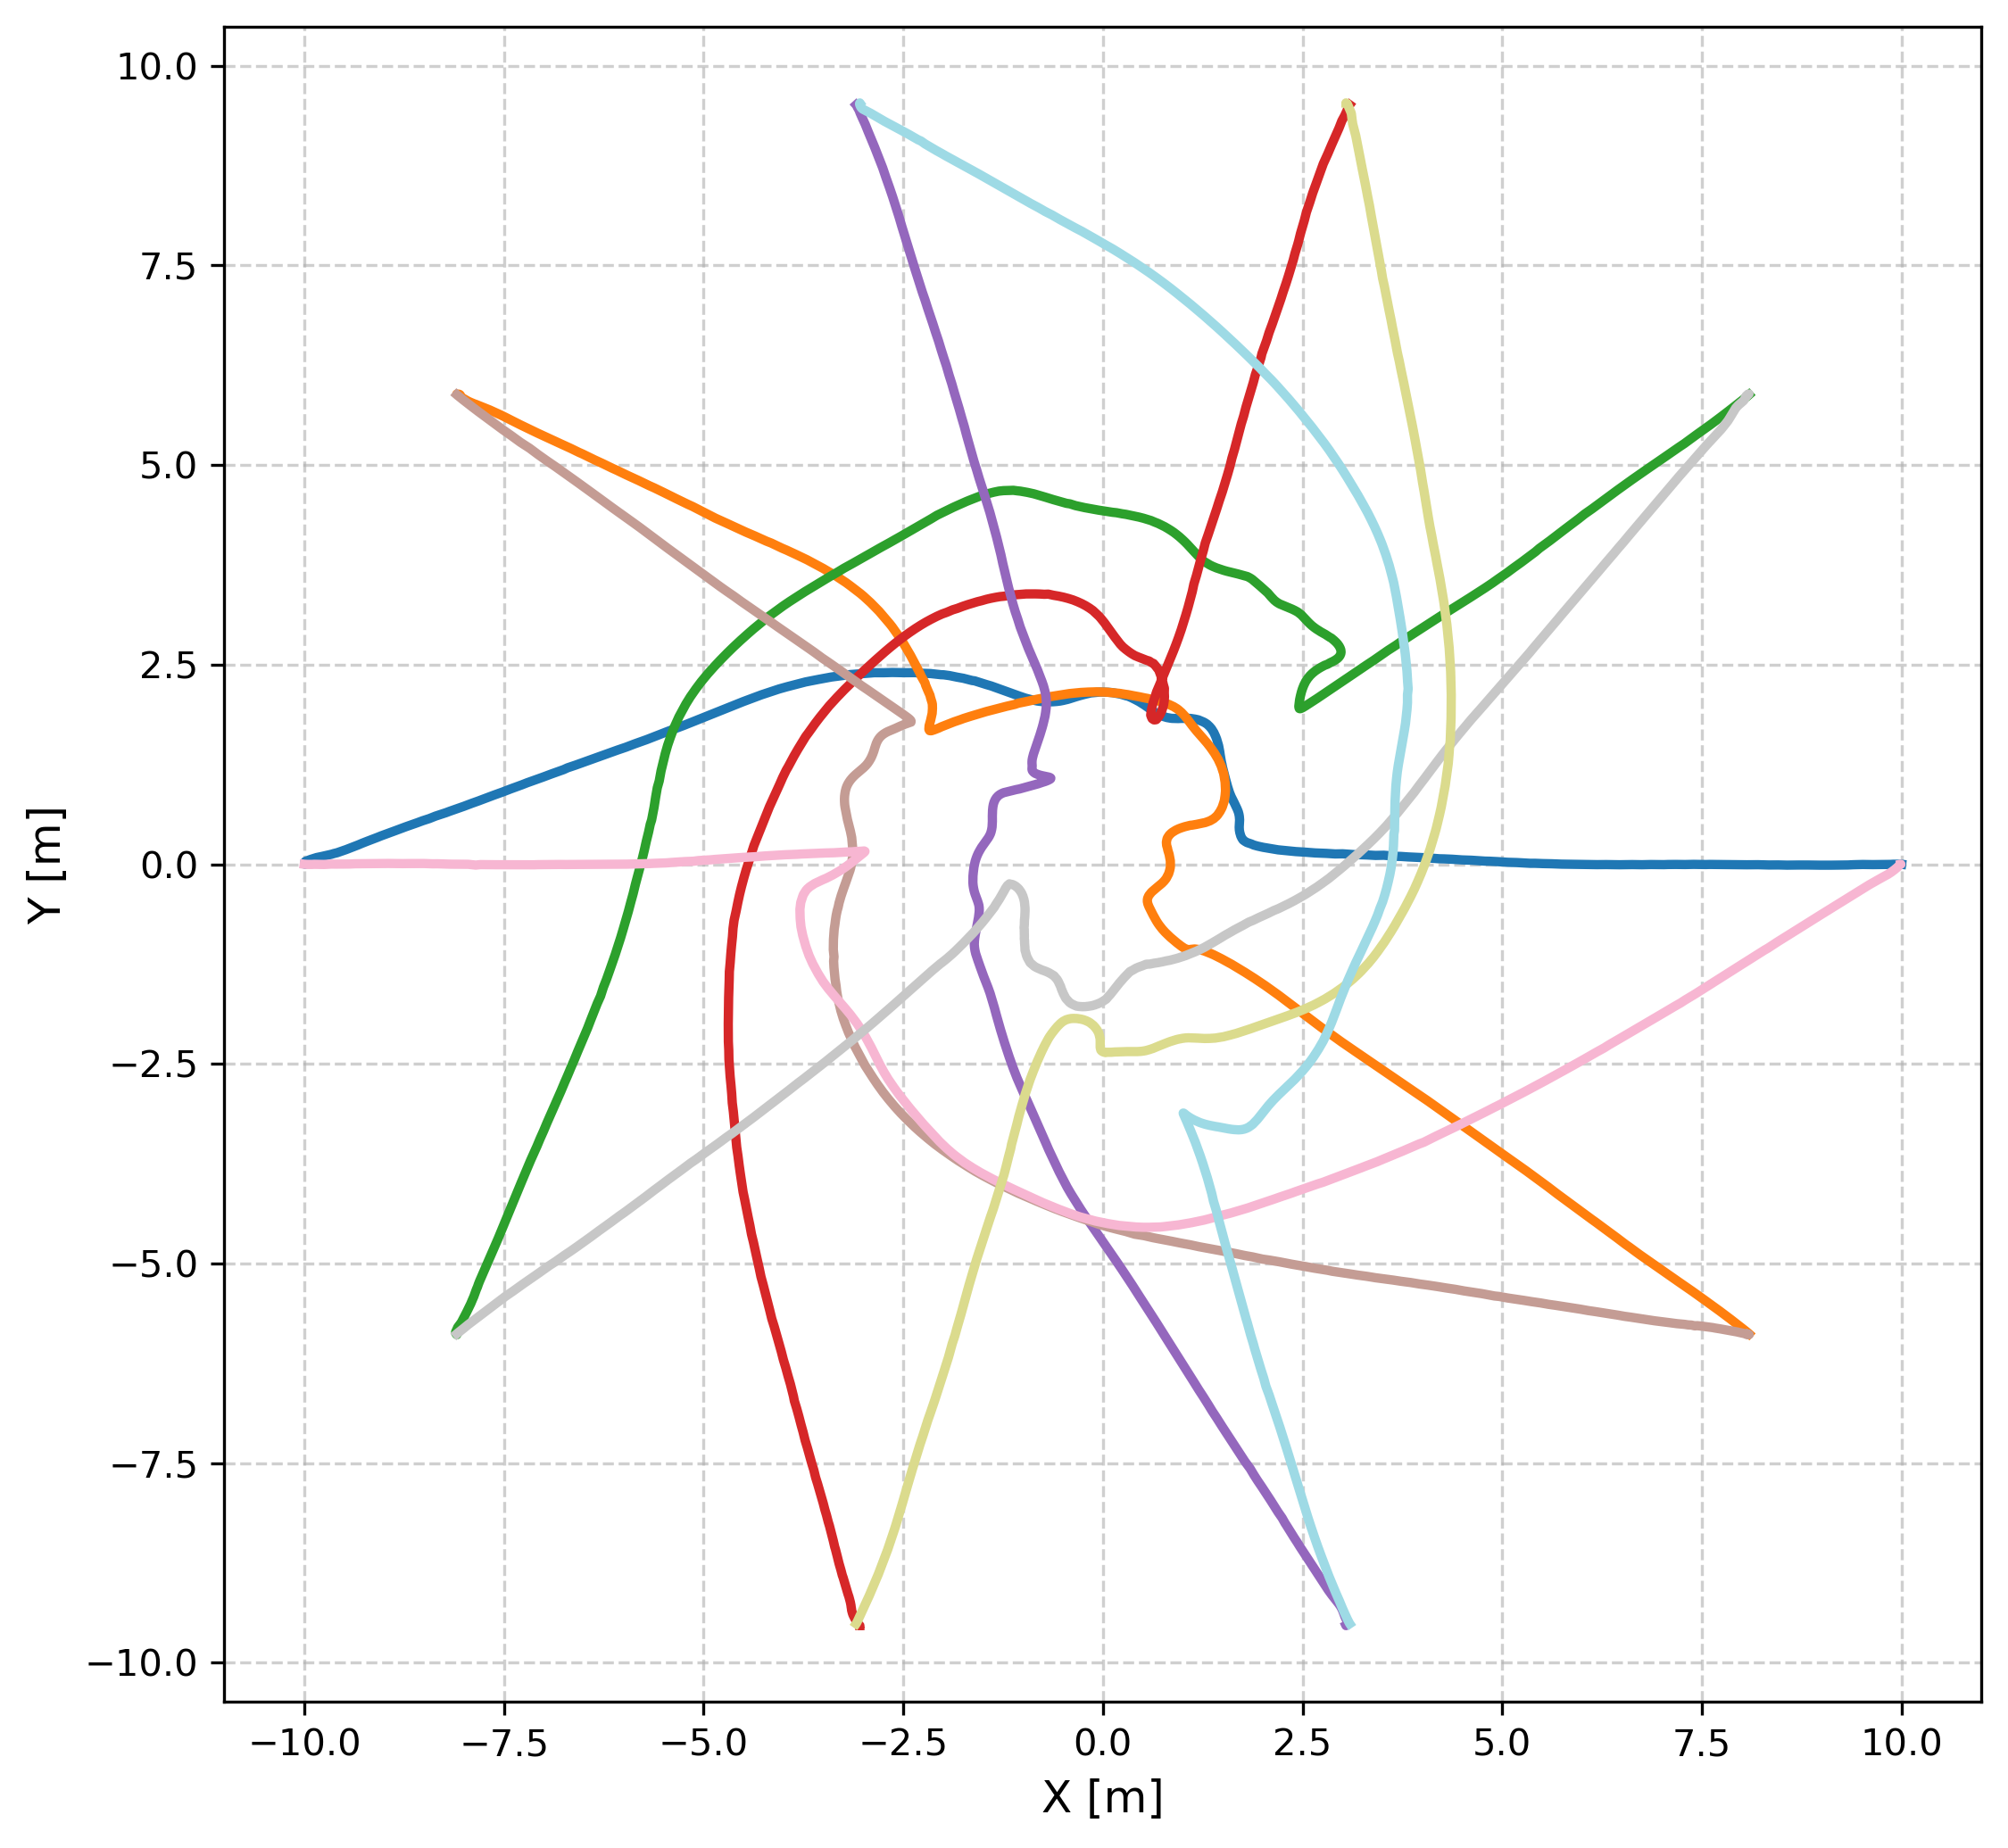
\includegraphics[width=0.48\textwidth, height=0.48\textwidth]{./fig/plots/circle_2d_top_down.png}
        }
        \subfloat[Side View (X-Z)] {
            \raisebox{0.12\textwidth}{
                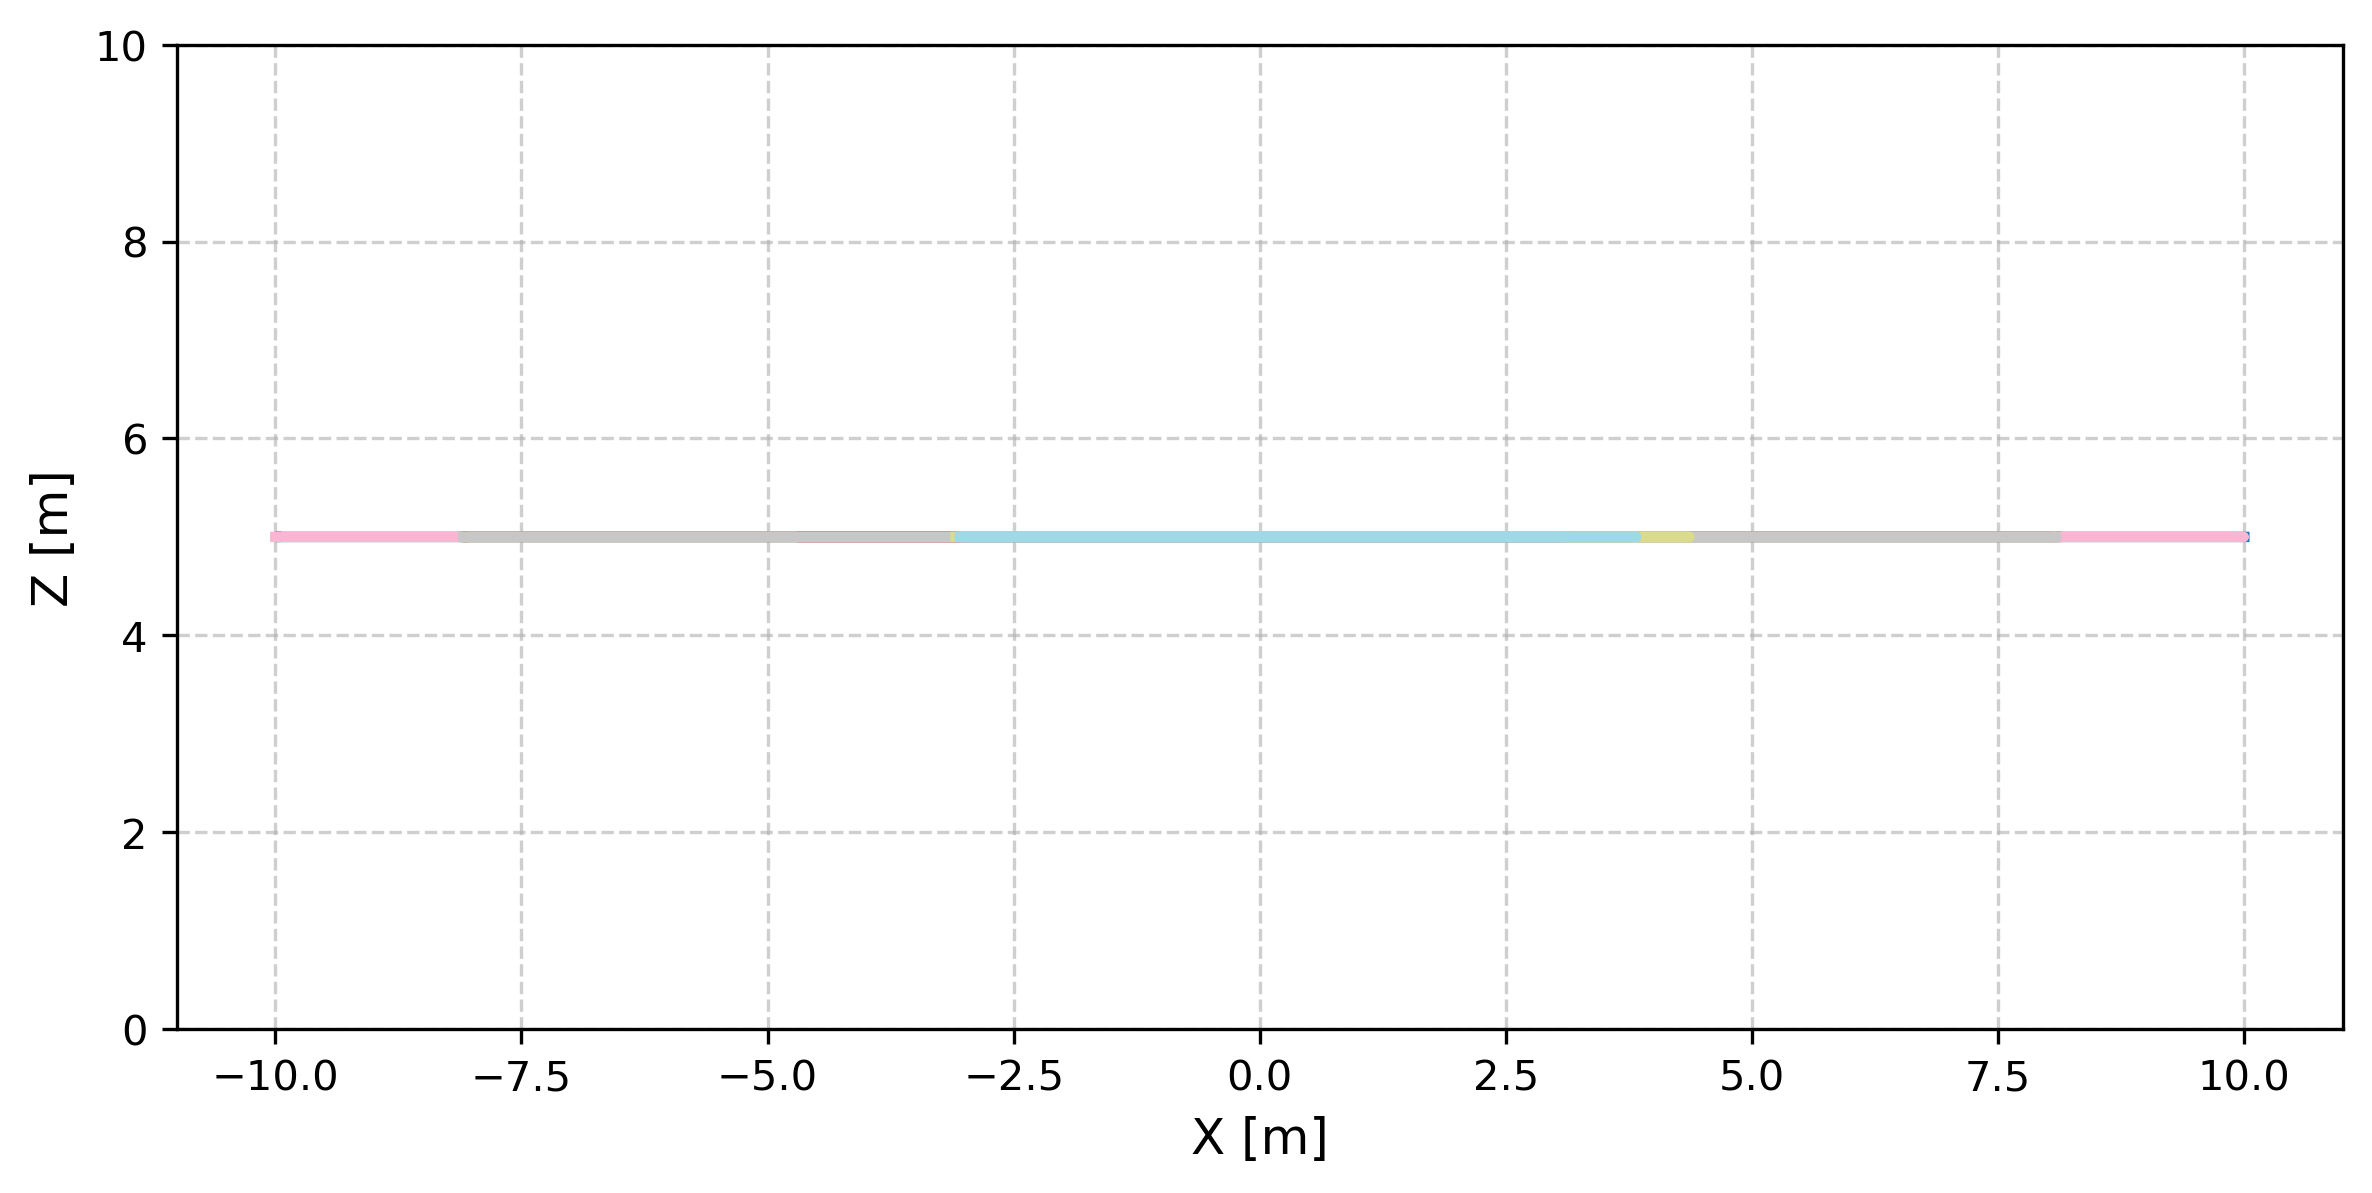
\includegraphics[width=0.48\textwidth, height=0.24\textwidth]{./fig/plots/circle_2d_side.png}
            }
        }
        \caption{
            Trajectories in a 2D circular crossing.
        }
        \label{}
    \end{figure}

    \begin{figure}[H]
        \centering
        \subfloat[Top-Down View (X-Y)] {
        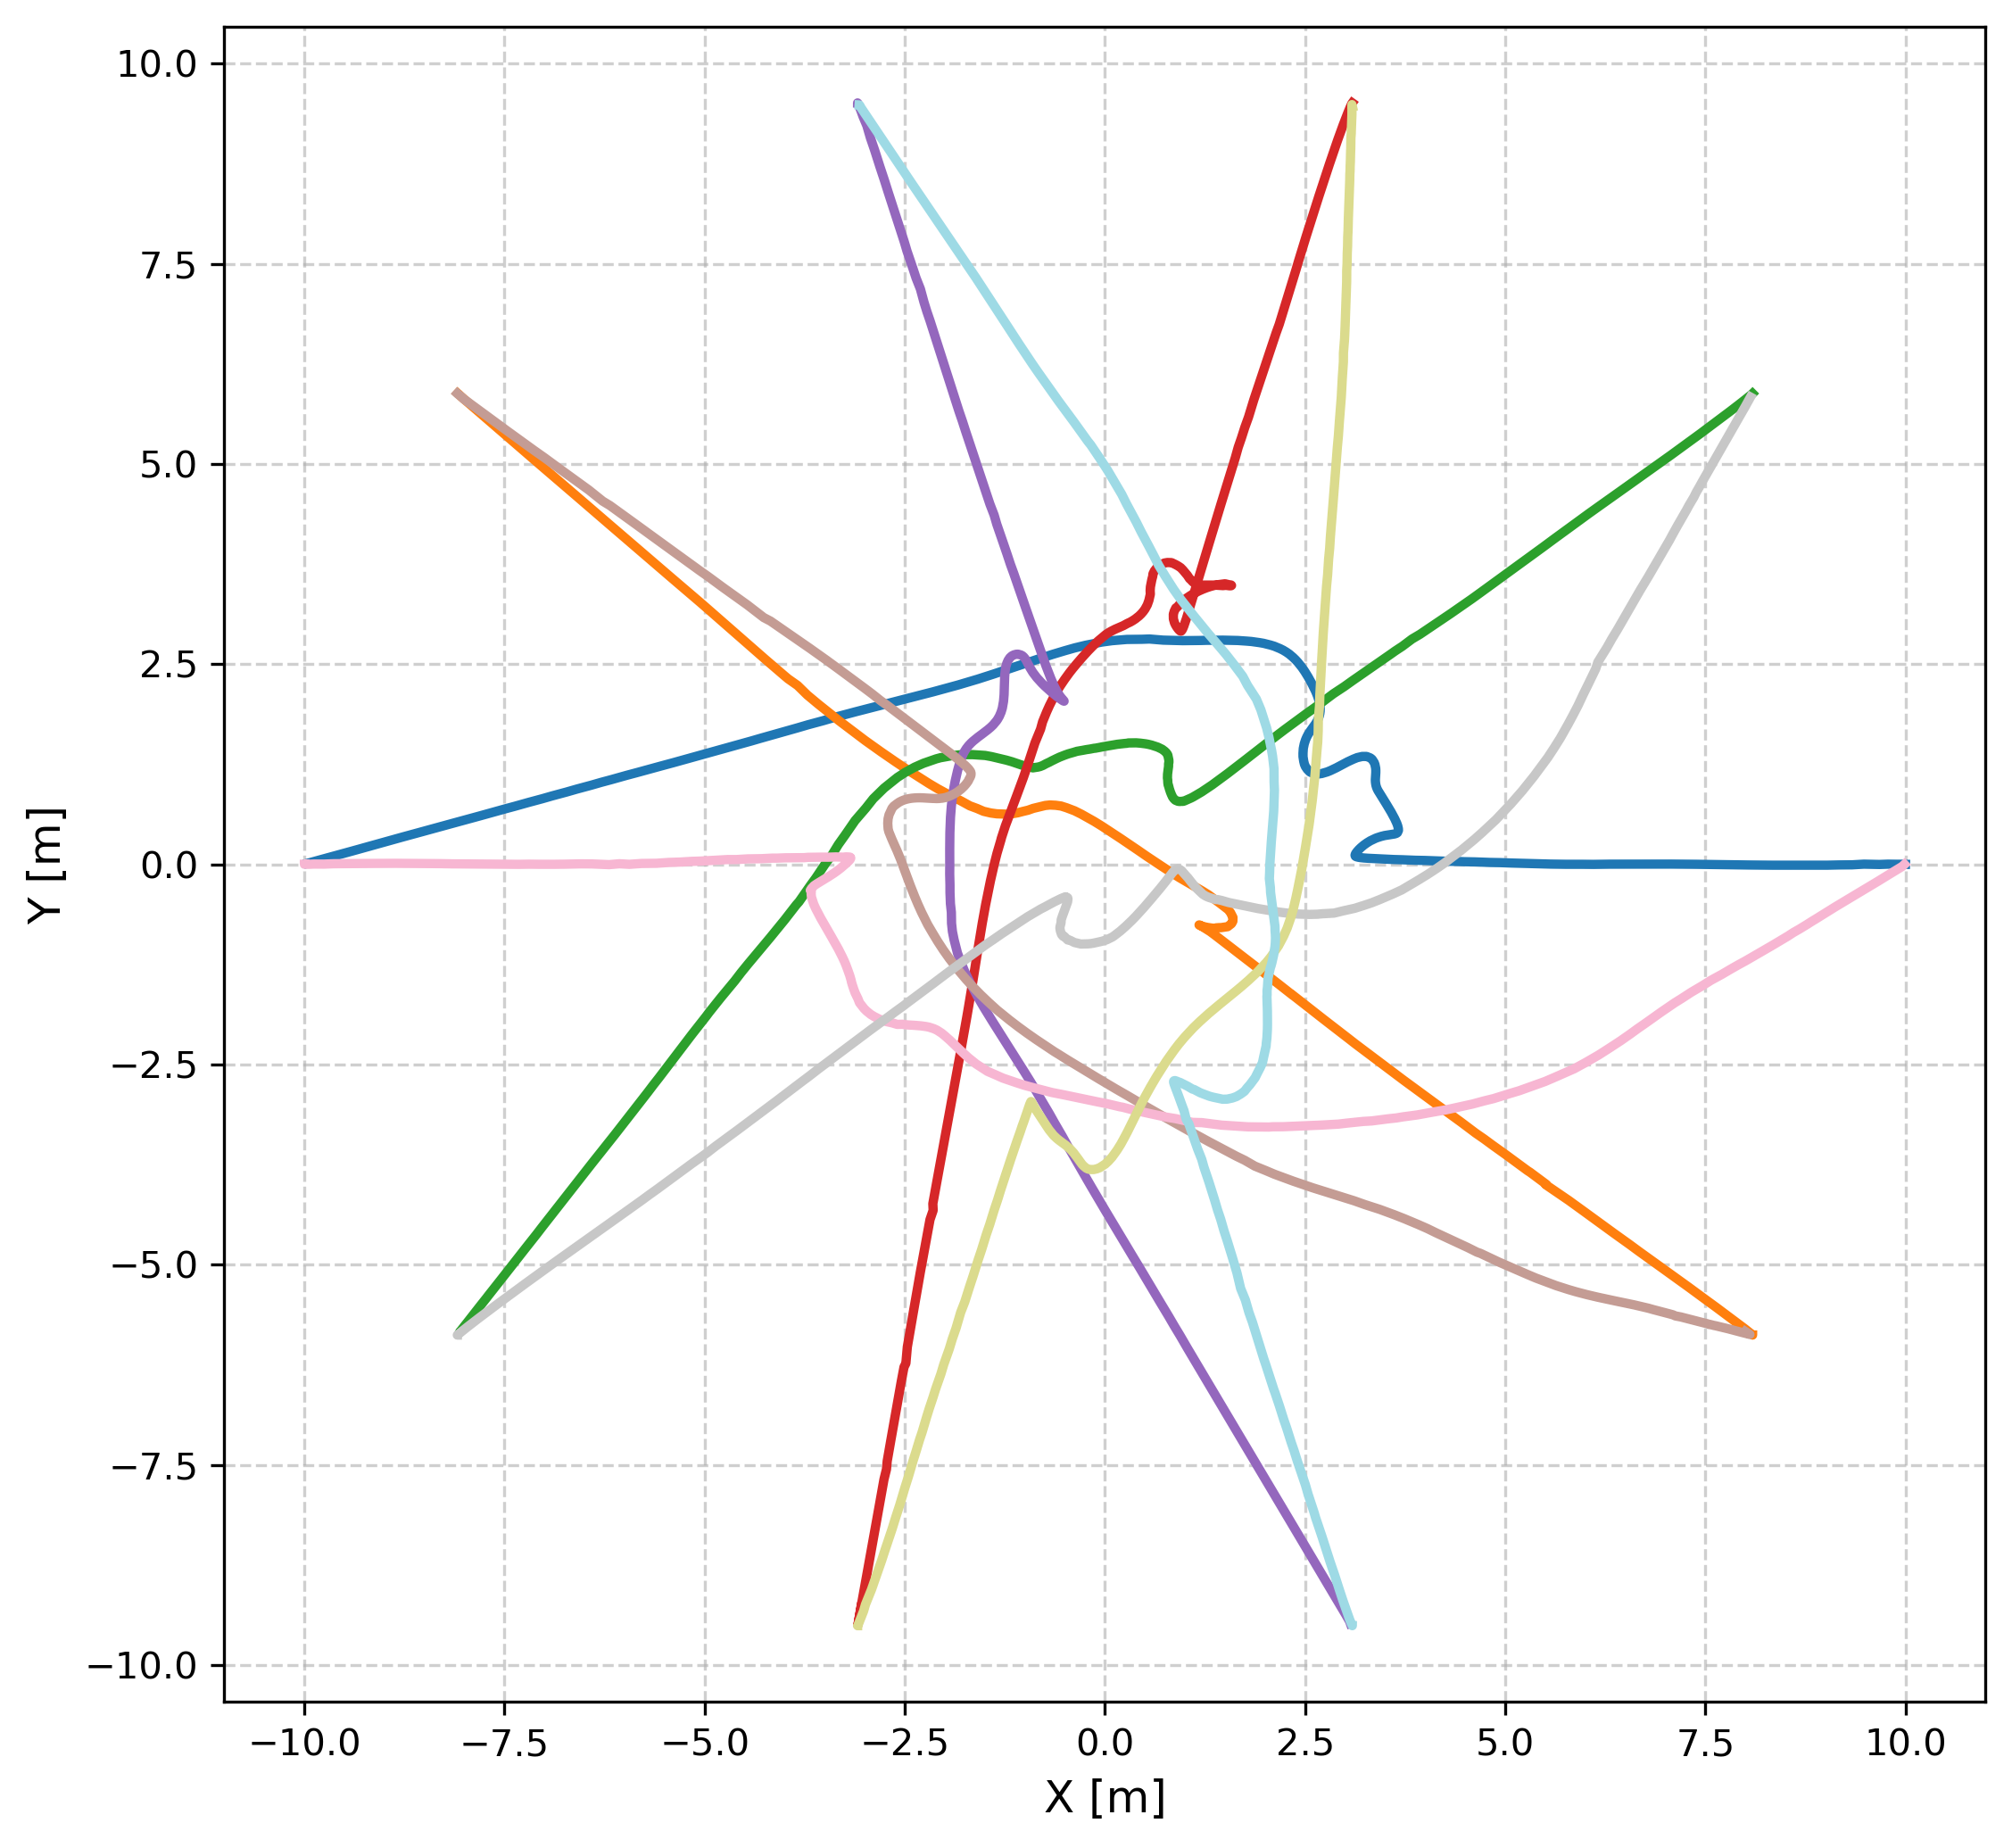
\includegraphics[width=0.48\textwidth, height=0.48\textwidth]{./fig/plots/circle_3d_top_down.png}
        }
        \subfloat[Side View (X-Z)] {
            \raisebox{0.12\textwidth}{
                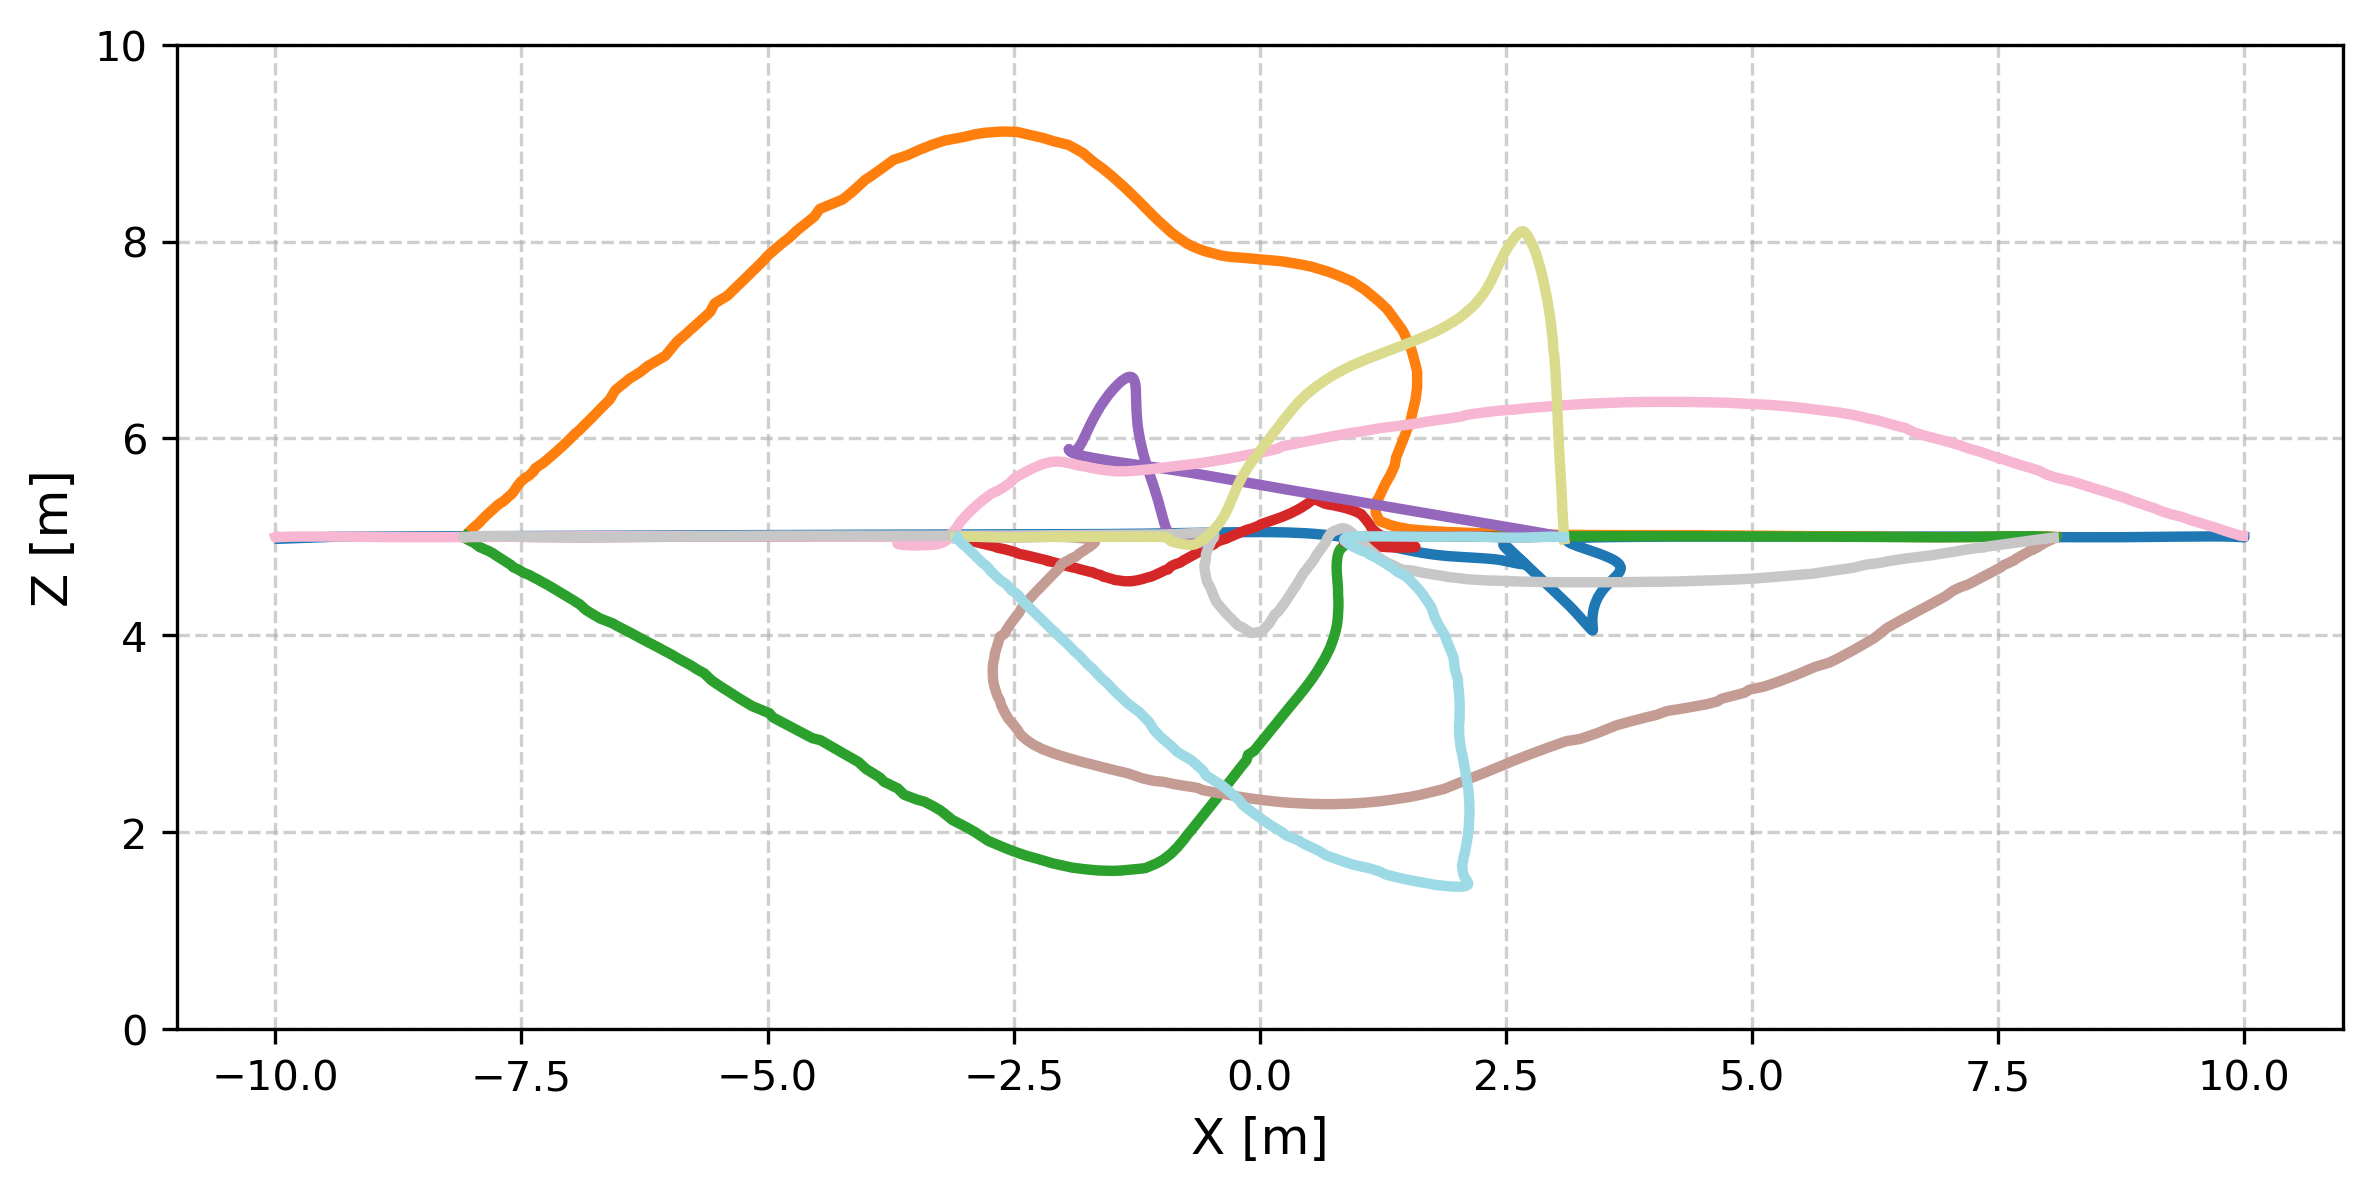
\includegraphics[width=0.48\textwidth, height=0.24\textwidth]{./fig/plots/circle_3d_side.png}
            }
        }
        \caption{
            Trajectories in a 3D circular crossing.
        }
        \label{}
    \end{figure}

    \begin{figure}[H]
        \centering
        \subfloat[Top-Down View (X-Y)] {
        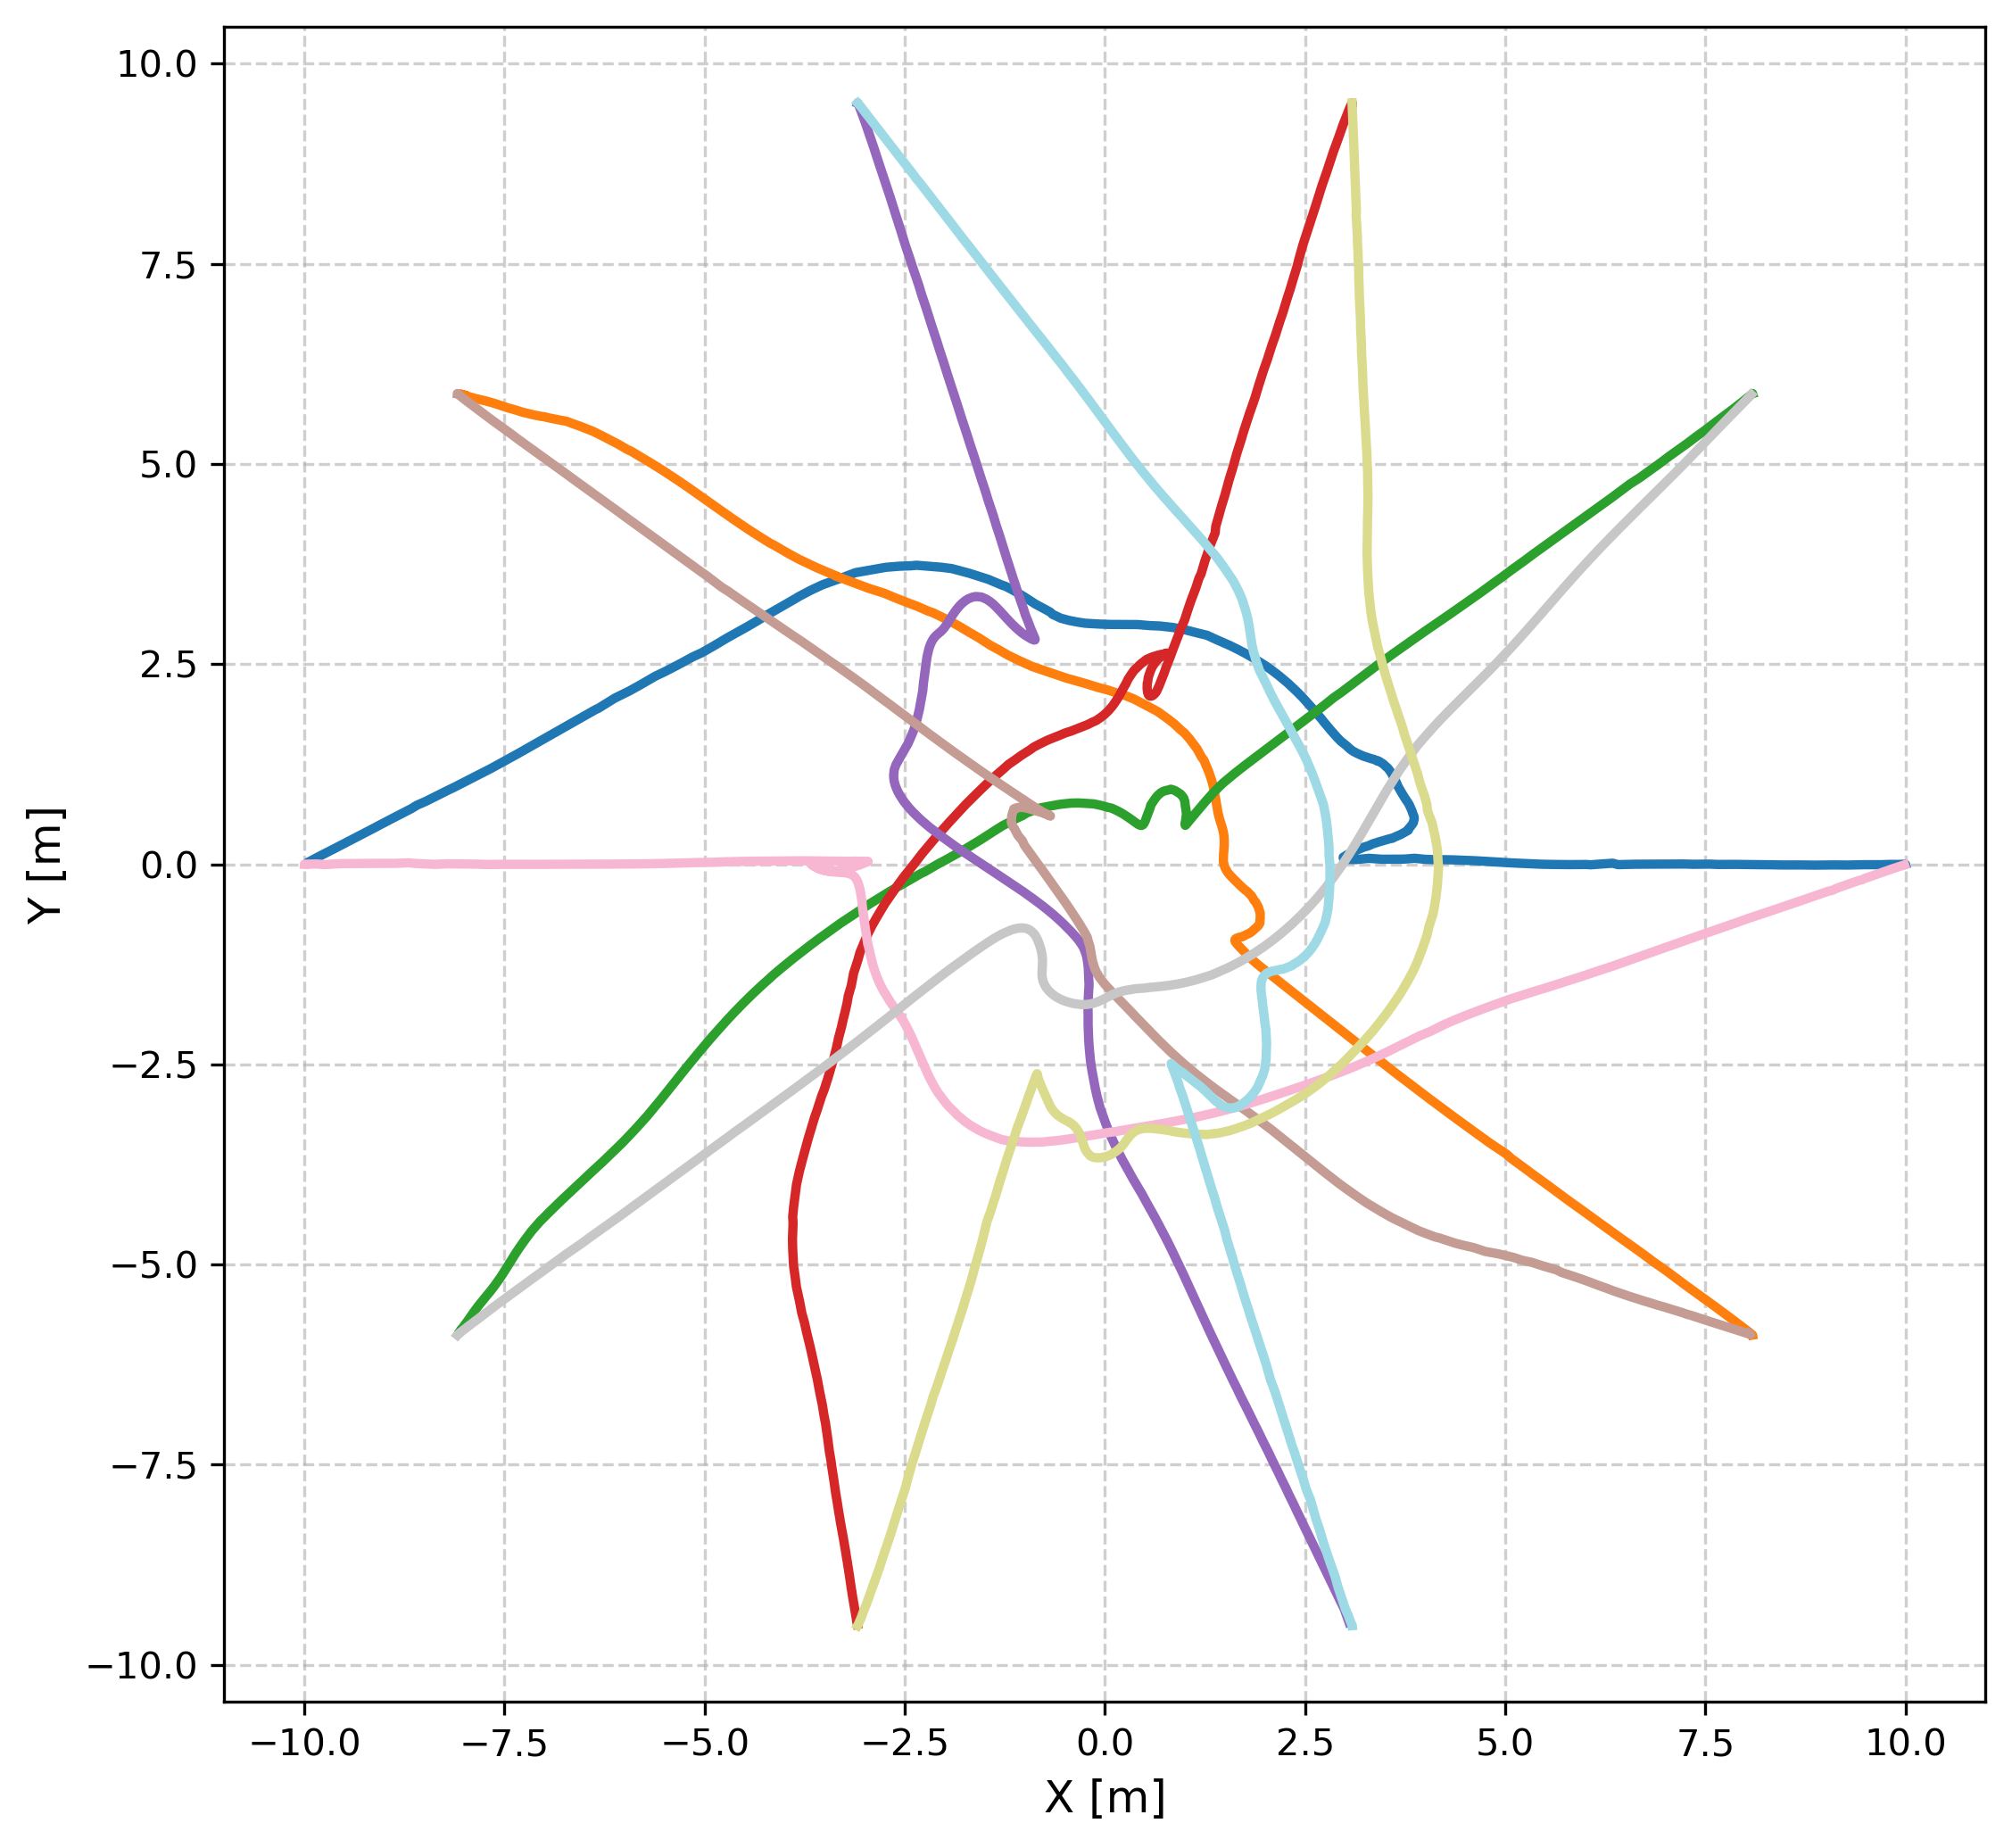
\includegraphics[width=0.48\textwidth, height=0.48\textwidth]{./fig/plots/circle_3d_z_clip_top_down.png}
        }
        \subfloat[Side View (X-Z)] {
            \raisebox{0.12\textwidth}{
                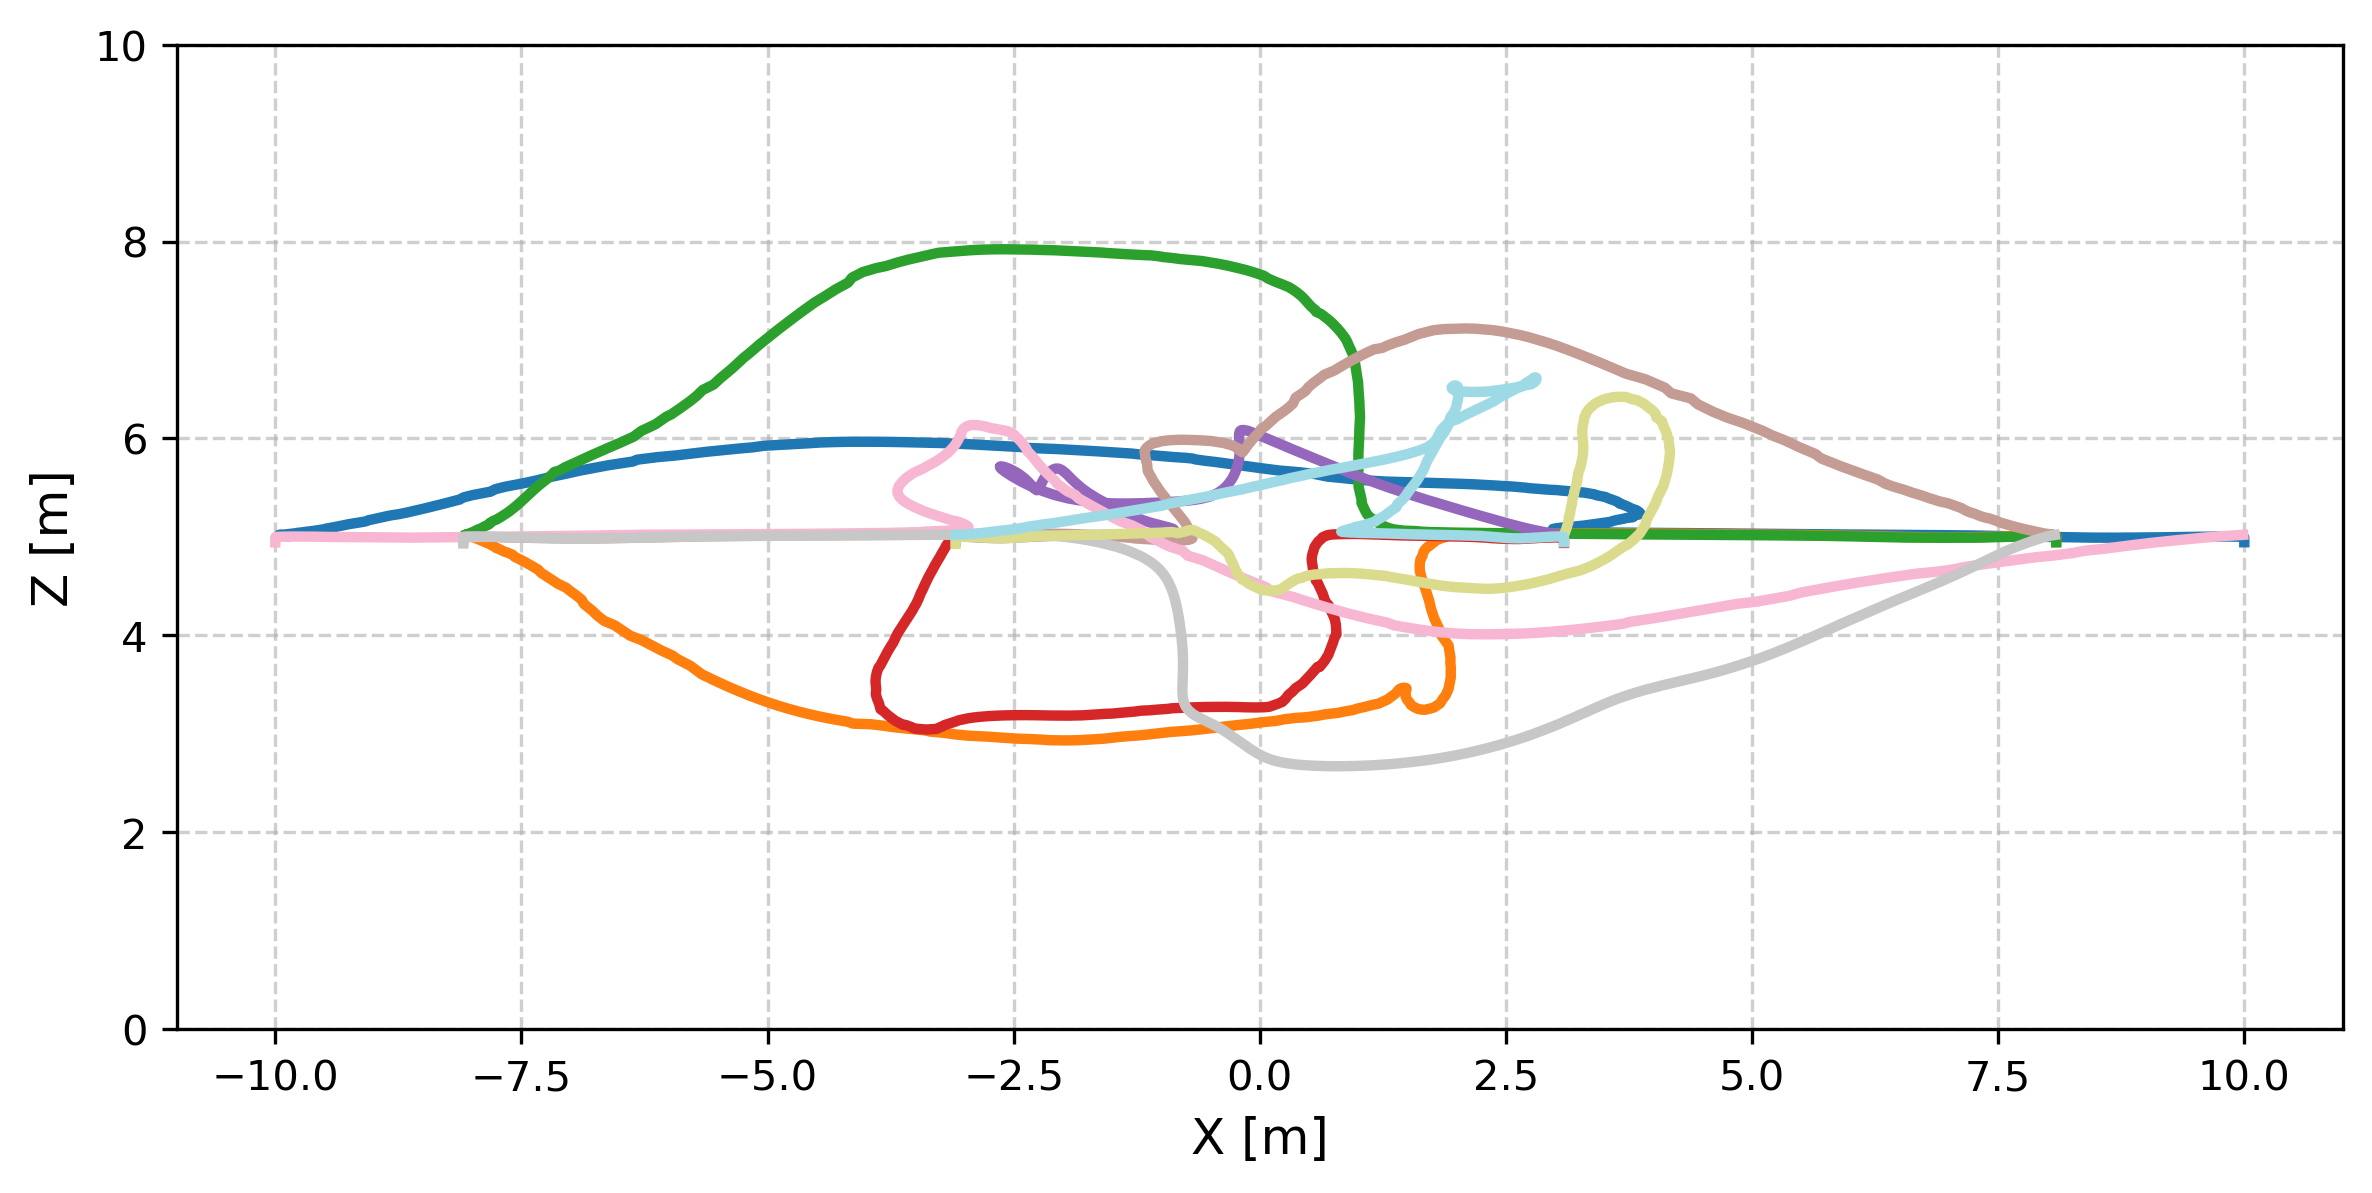
\includegraphics[width=0.48\textwidth, height=0.24\textwidth]{./fig/plots/circle_3d_z_clip_side.png}
            }
        }
        \caption{
            Effect of Z-axis clipping on the circular crossing.   
        }
        \label{}
    \end{figure}

    \begin{figure}[H]
        \centering
        \subfloat[Top-Down View (X-Y)] {
        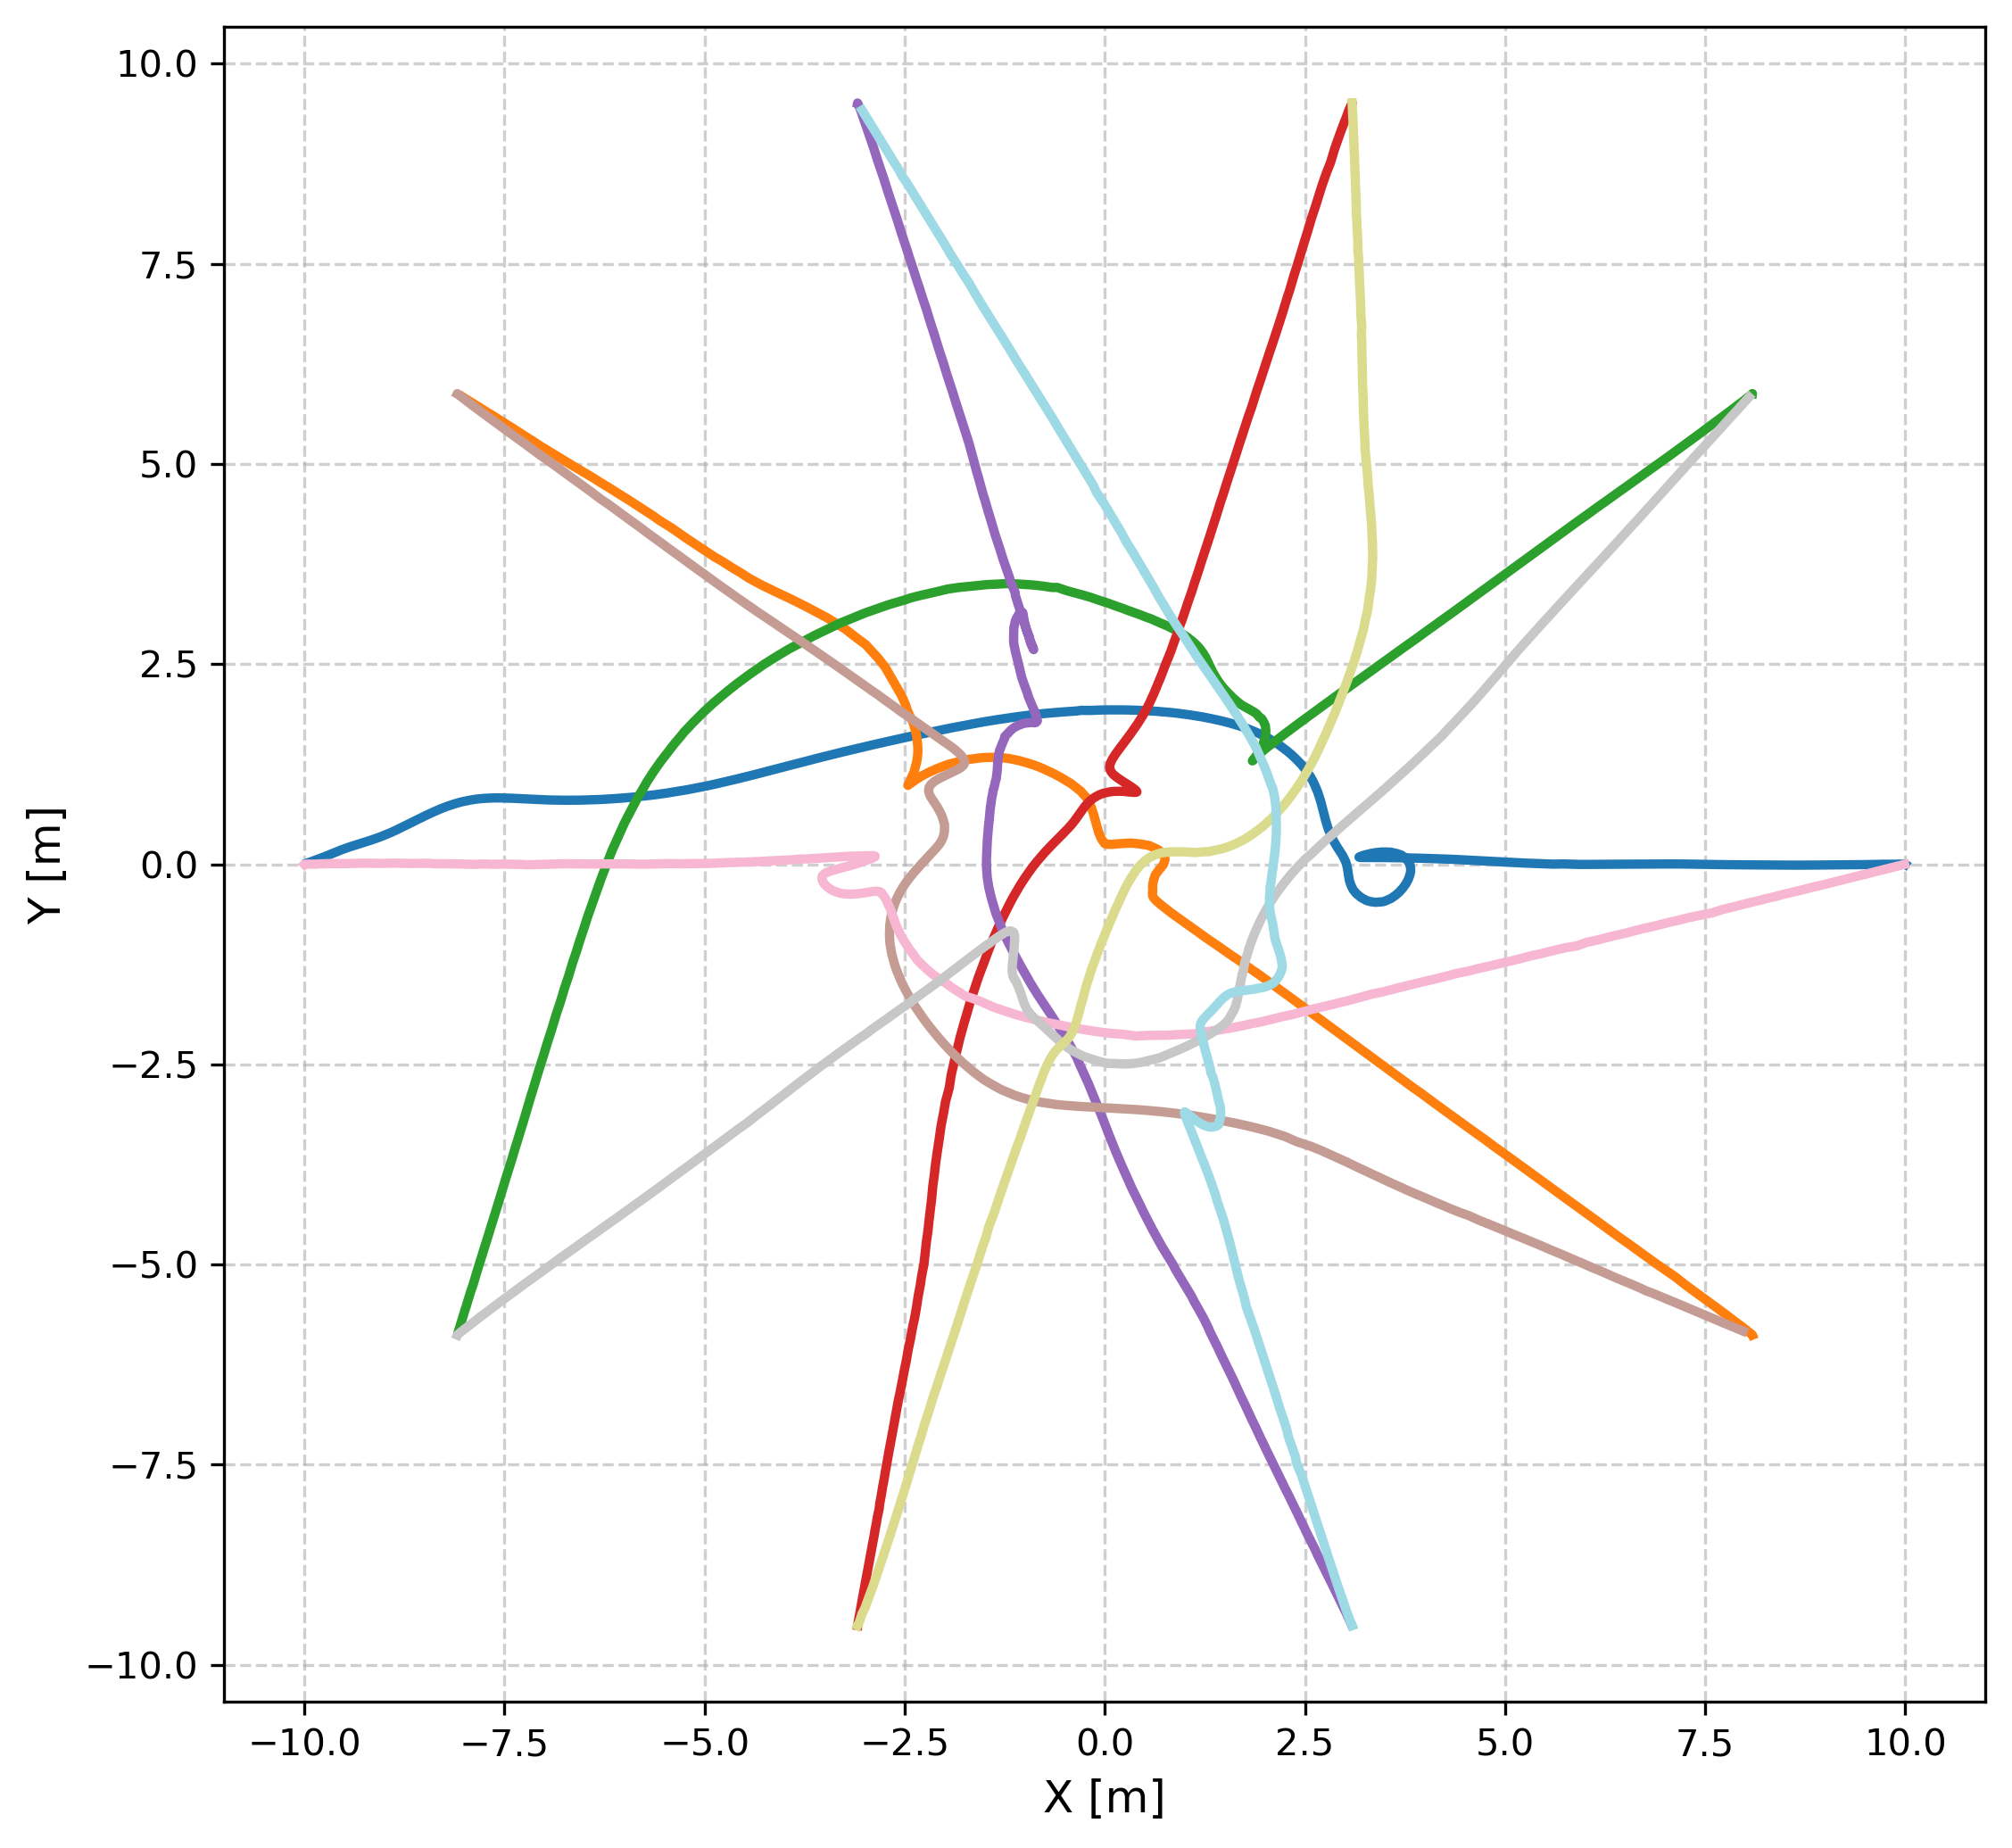
\includegraphics[width=0.48\textwidth, height=0.48\textwidth]{./fig/plots/circle_3d_z_rule_top_down.png}
        }
        \subfloat[Side View (X-Z)] {
            \raisebox{0.12\textwidth}{
                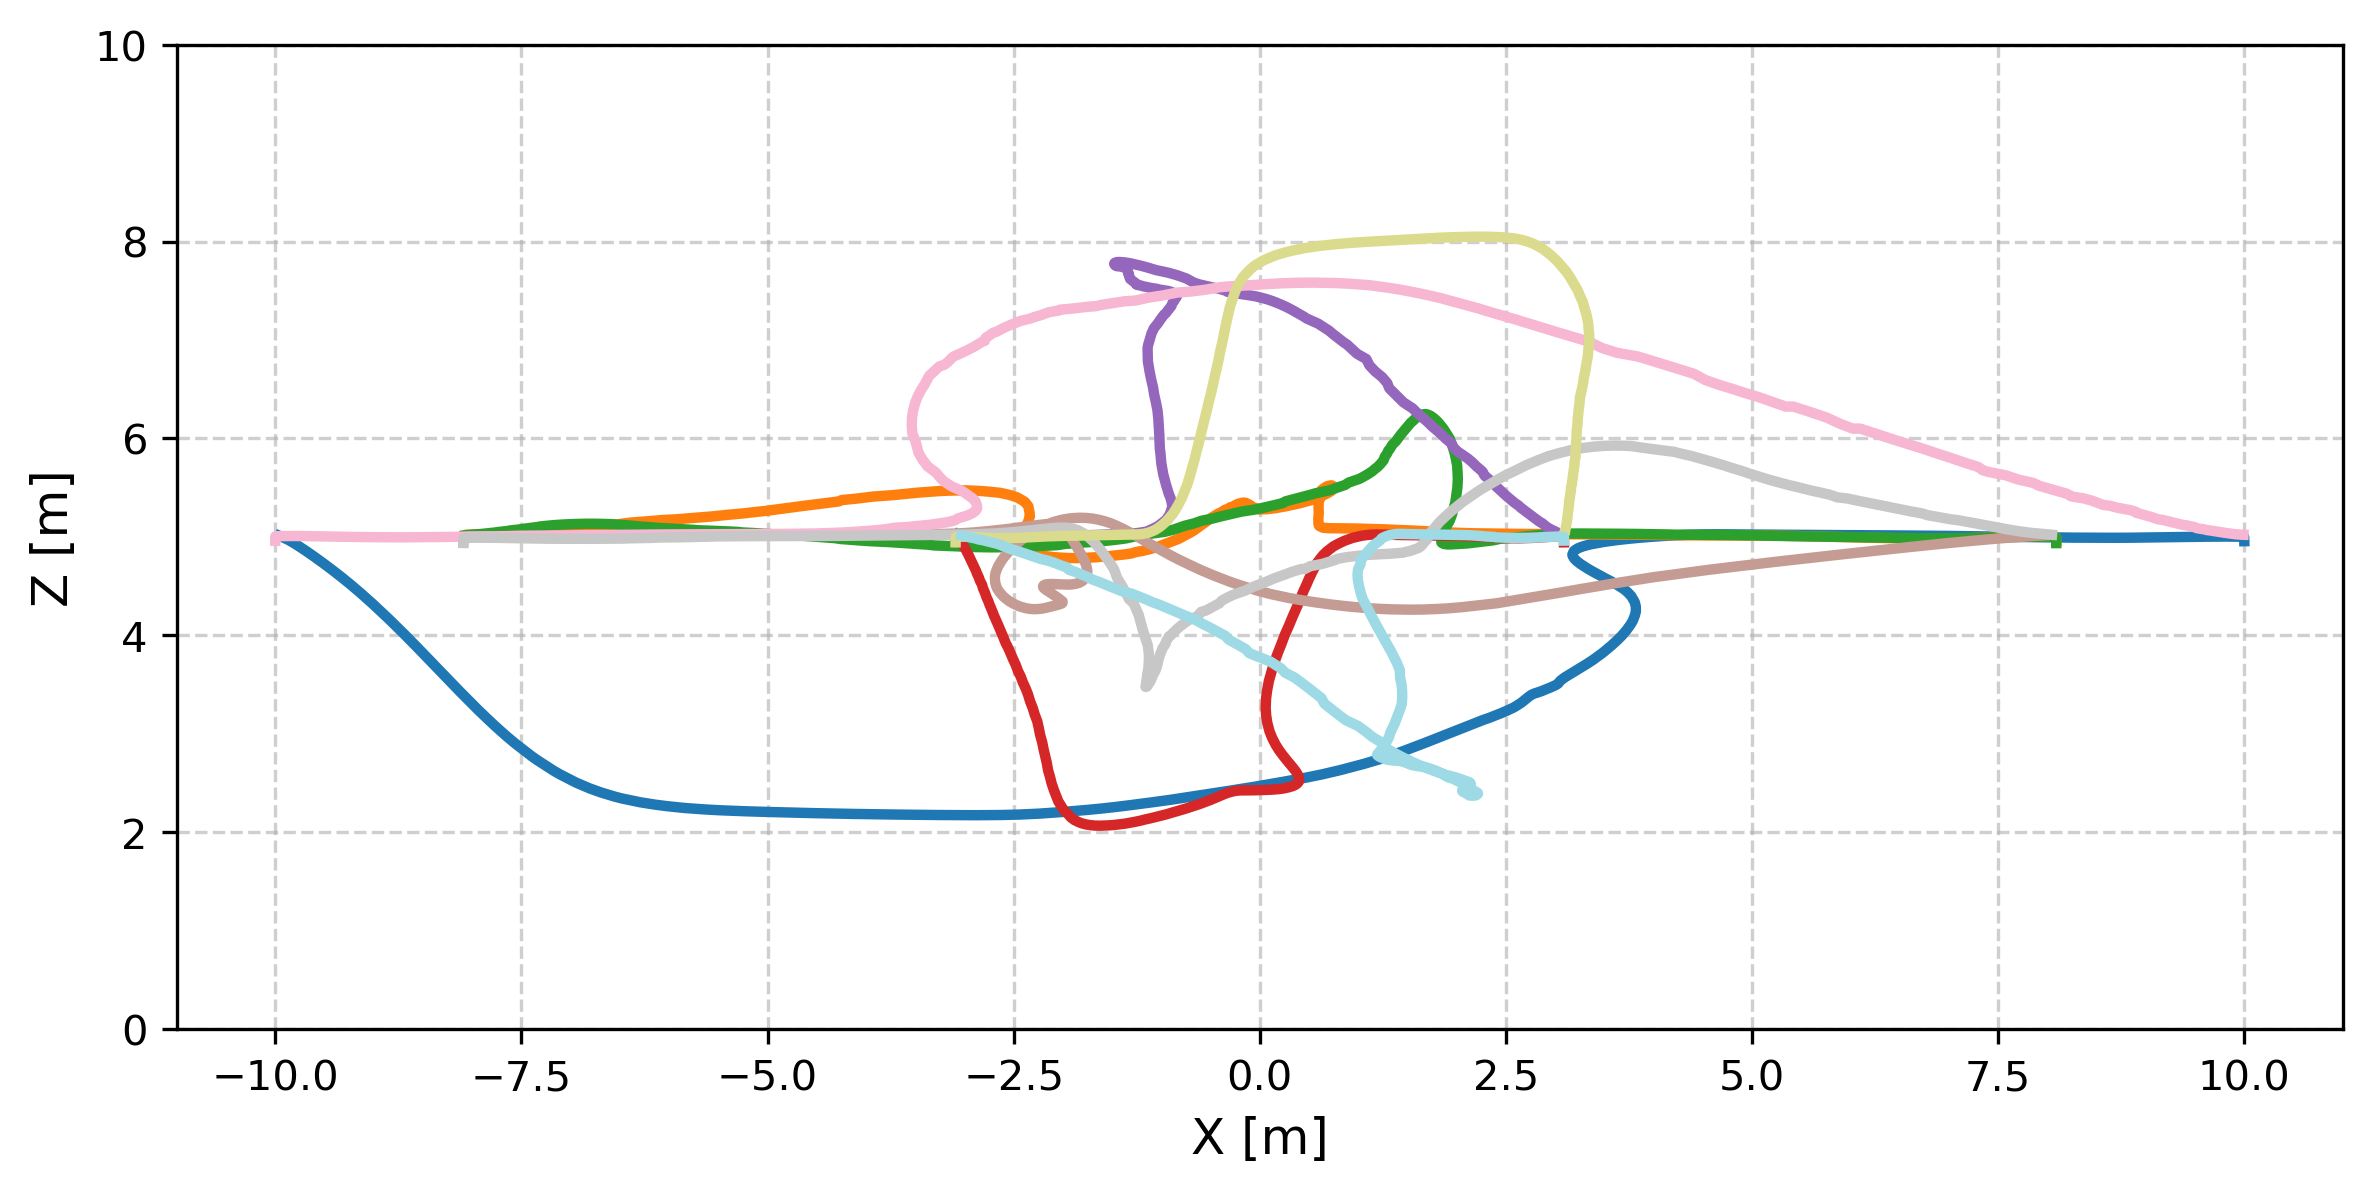
\includegraphics[width=0.48\textwidth, height=0.24\textwidth]{./fig/plots/circle_3d_z_rule_side.png}
            }
        }
        \caption{
            Effect of the Z-axis rule on the circular crossing. 
        }
        \label{}
    \end{figure}

    \begin{figure}[H]
        \centering
        \subfloat[Top-Down View (X-Y)] {
        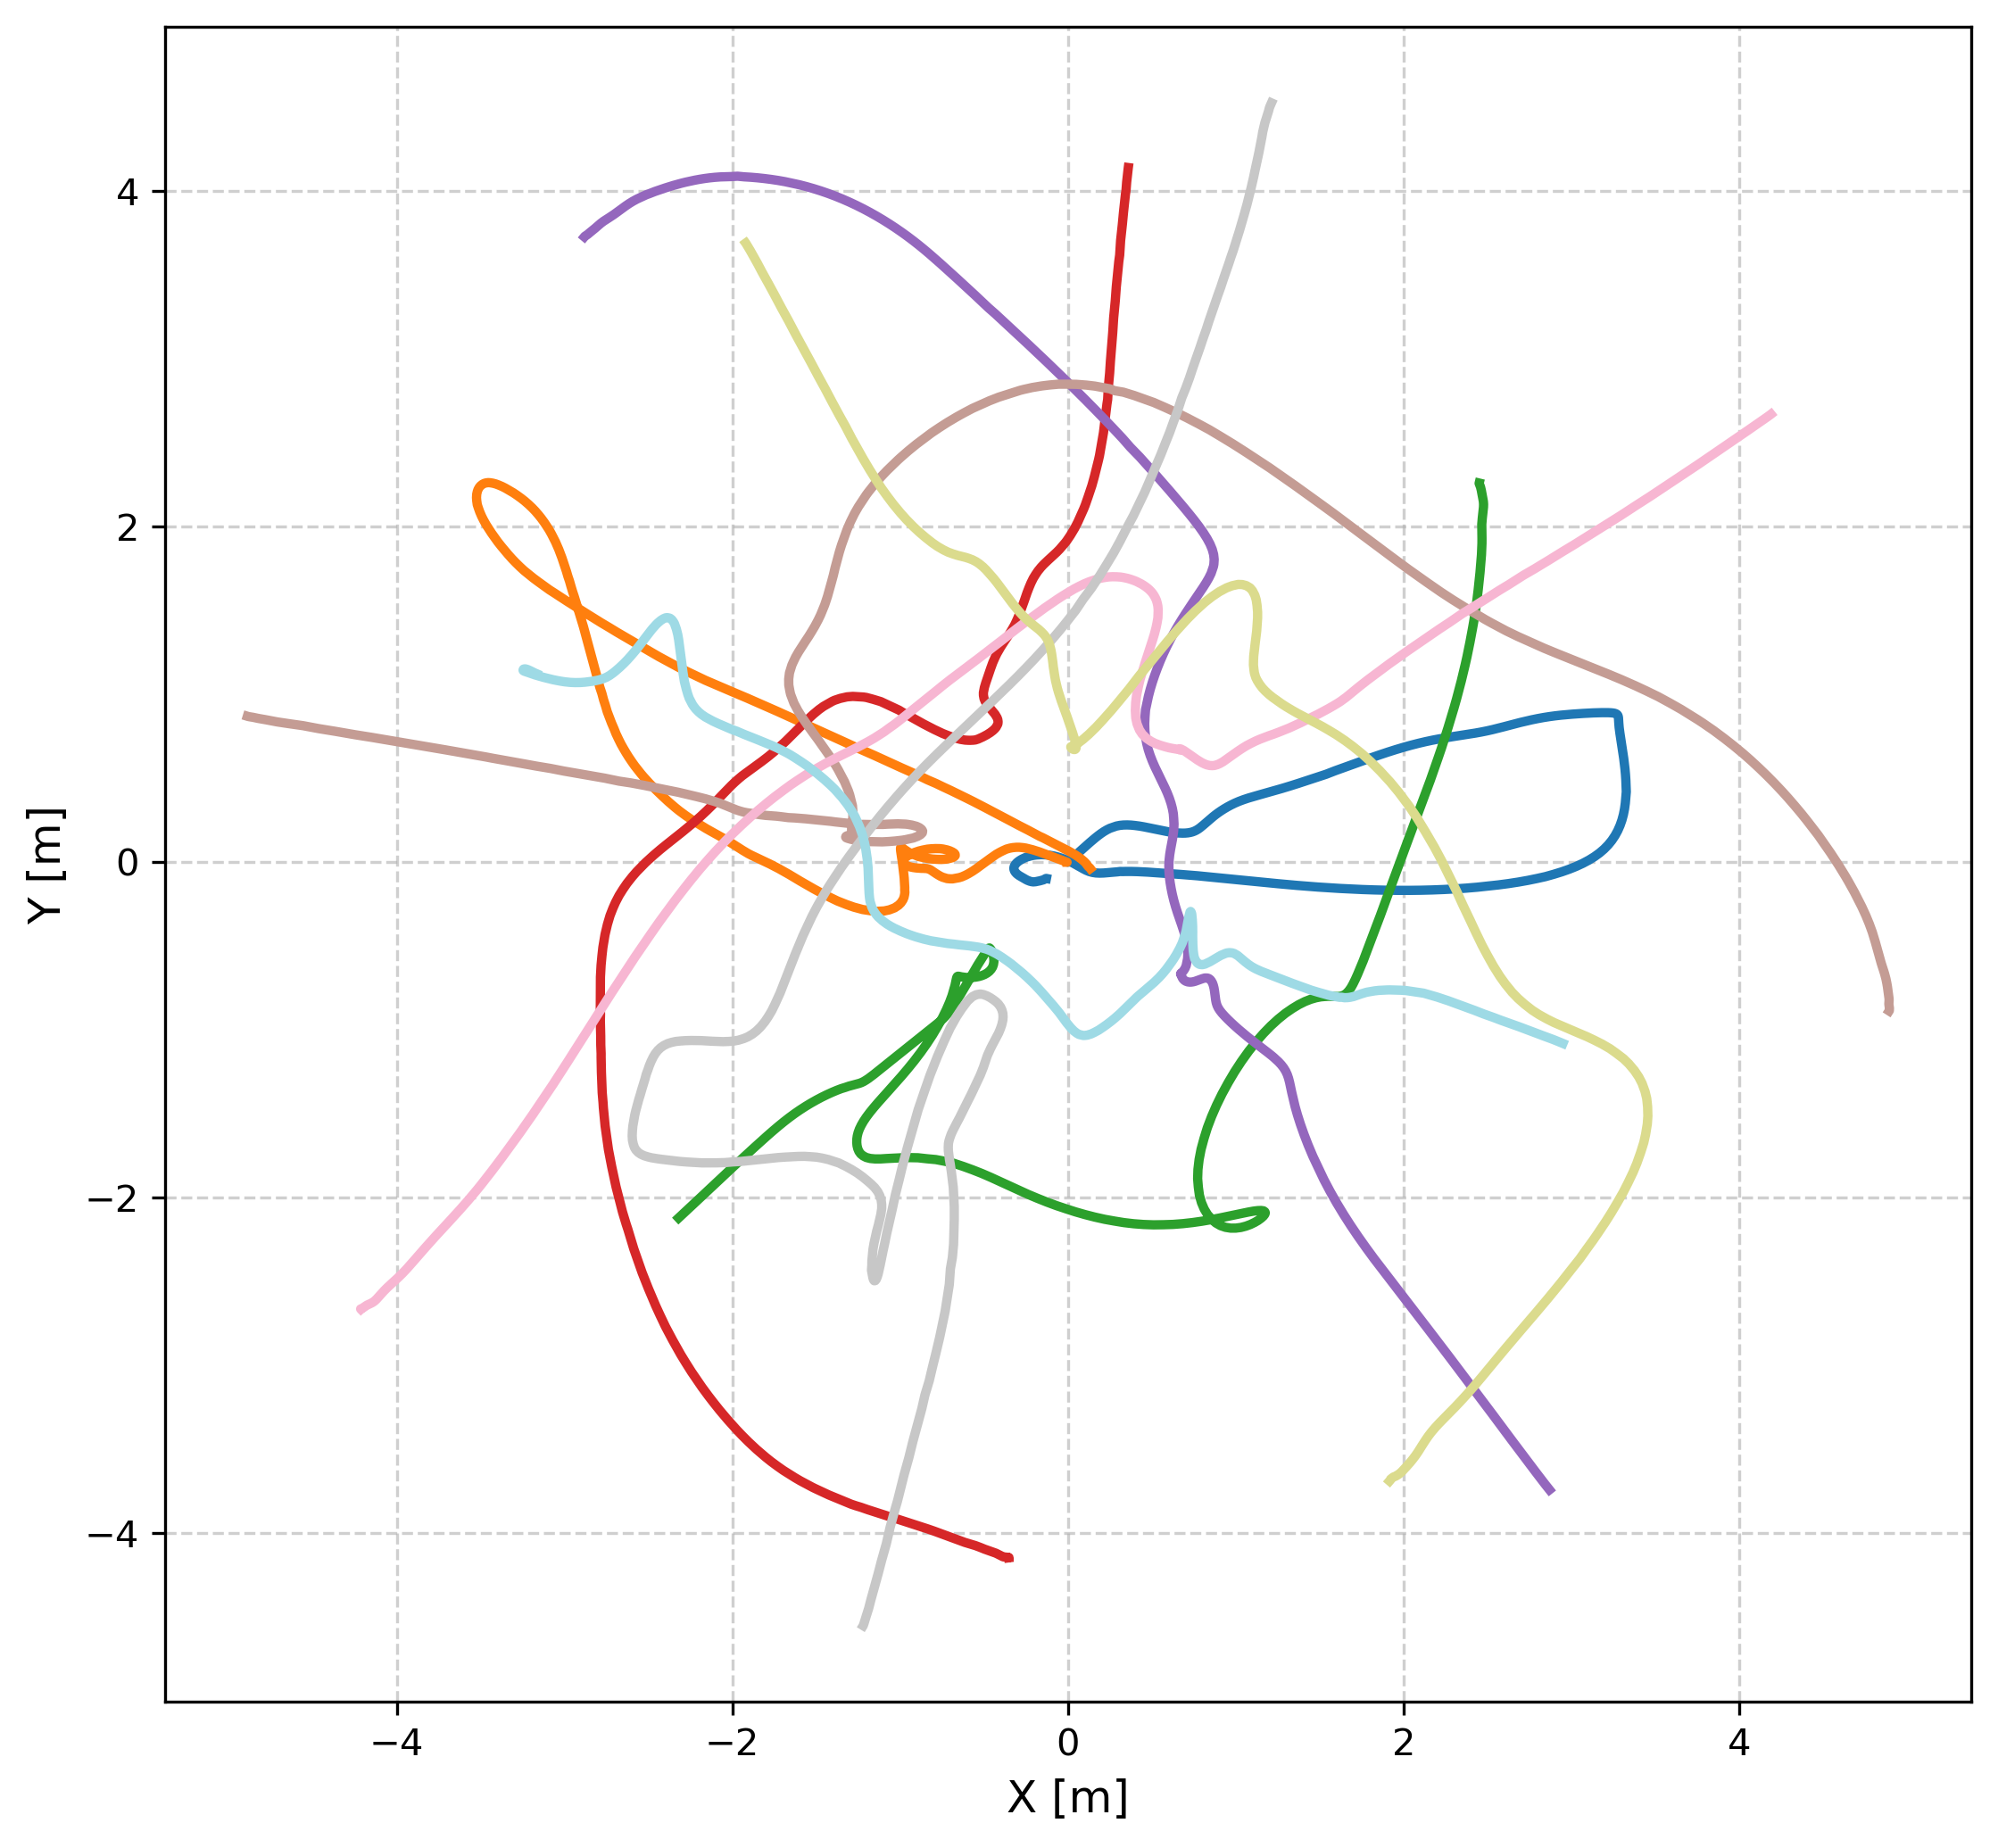
\includegraphics[width=0.48\textwidth, height=0.48\textwidth]{./fig/plots/sphere_3d_top_down.png}
        }
        \subfloat[Side View (X-Z)] {
        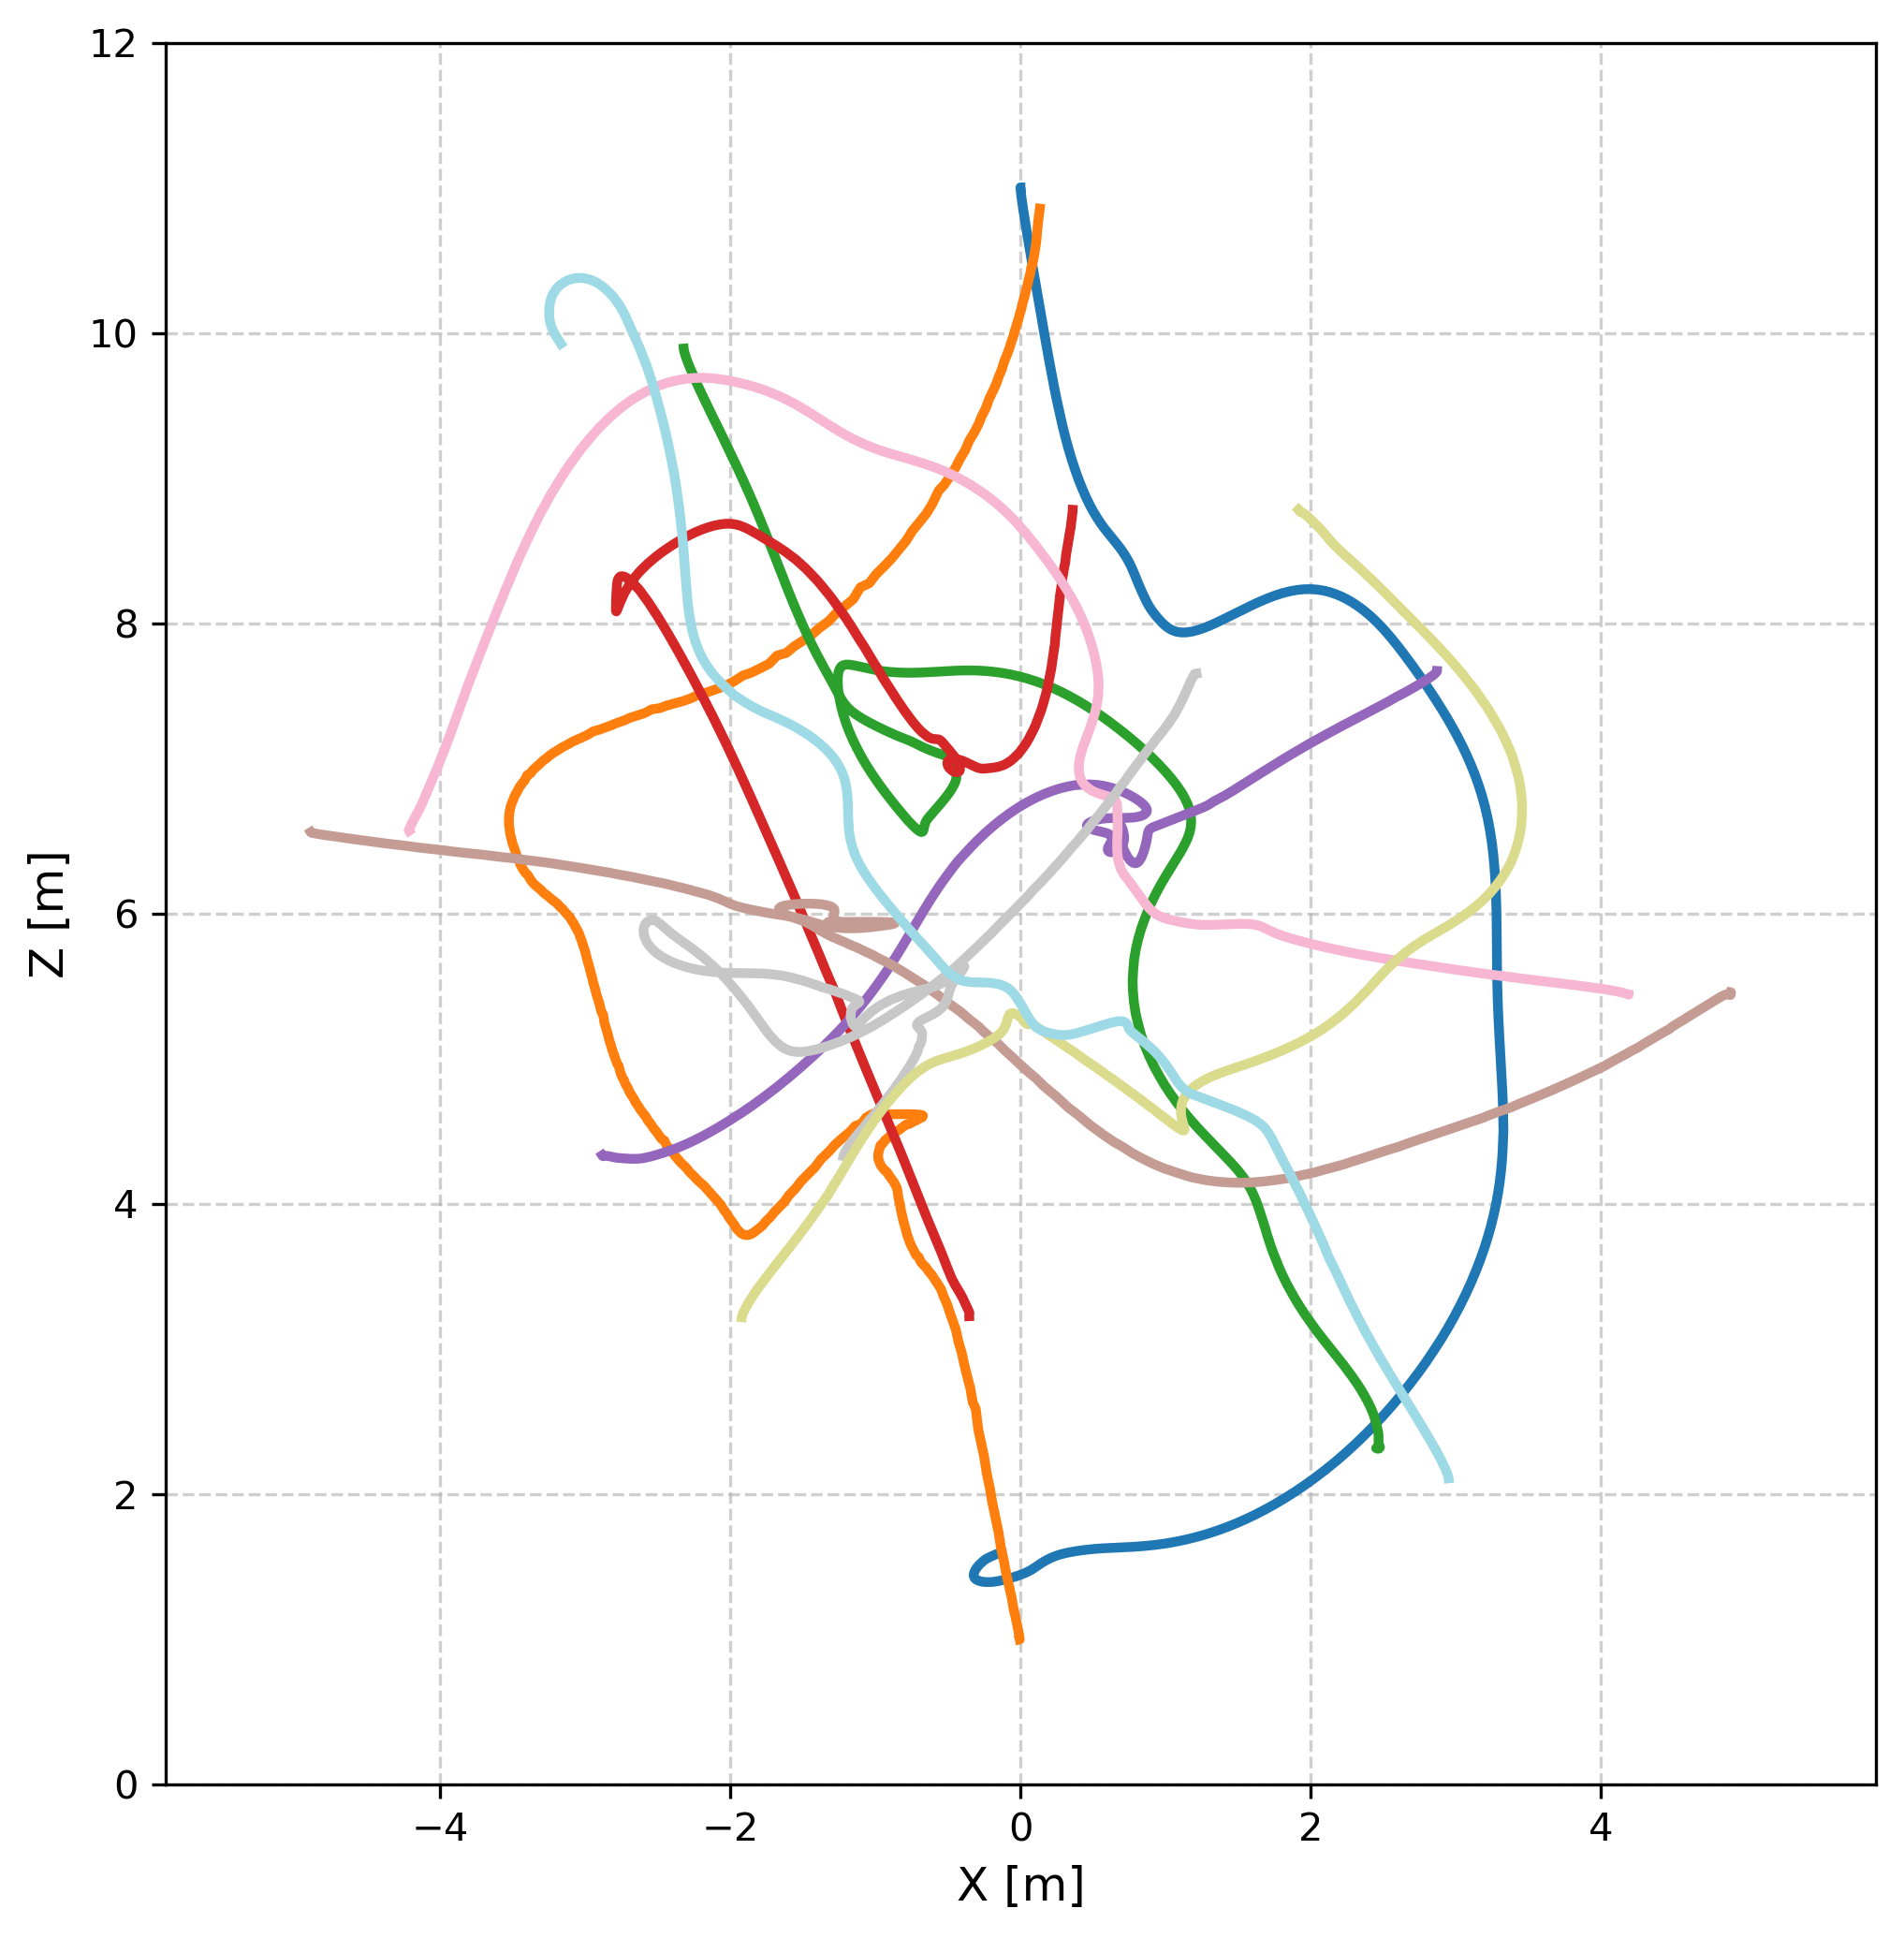
\includegraphics[width=0.48\textwidth, height=0.48\textwidth]{./fig/plots/sphere_3d_side.png}
        }
        \caption{
            Trajectories in a 3D spherical crossing.
        }
        \label{}
    \end{figure}